\documentclass{article}
\usepackage[utf8]{inputenc}
\usepackage[margin=1in]{geometry}
\usepackage{amsmath}
\usepackage{amsthm}
\usepackage{hyperref}
\usepackage{cancel}
% Package for making turing machine diagrams %
\usepackage{tikz}
\usetikzlibrary{chains,fit,shapes}
% Packages for algorithms %
\usepackage{algorithm}
\usepackage{algorithmic}
% Package which has the nice looking empty set symbol (\varnothing)
\usepackage{amssymb}
% Package with the ceiling function
%\usepackage{mathtools}
%\DeclarePairedDelimiter{\ceil}{\lceil}{\rceil}
\usepackage{bm}
\usepackage{braket}
\usepackage{theoremref}
\usepackage{graphicx}
\graphicspath{{./images/}}

\theoremstyle{theorem}
\newtheorem{fact}{Fact}[section]
\newtheorem{lemma}{Lemma}[section]
\newtheorem{theorem}{Theorem}[section]
\newtheorem{corollary}{Corollary}[section]
\newtheorem{claim}{Claim}[section]
\newtheorem{conjecture}{Conjecture}[section]

\title{An Elaboration and Visualization of Morishima's Completion of Marx's Reproduction Schema}
\author{Alex Creiner}

\begin{document}
\maketitle
\href{https://www.desmos.com/calculator/wygiqzniwt}{\color{blue} \LARGE Click me to go to the app!} 
\begin{figure}[H]
\centering
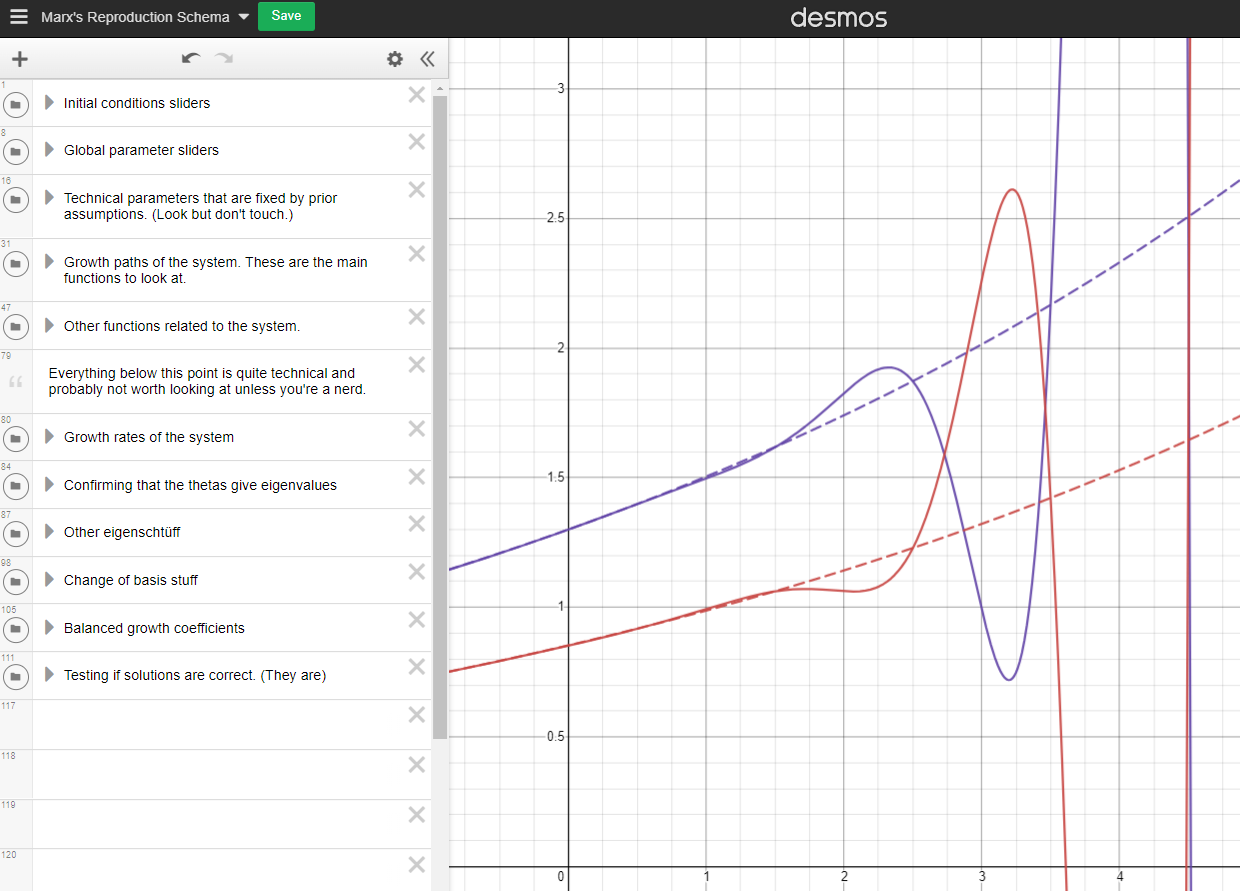
\includegraphics[scale=.5]{Images/introduction}
\caption{You should see something like this.}
\end{figure}
I made this to help myself understand some things a bit better, and found myself amazed how well it turned out and how easy it was to add in lots bells and whistles allowing us to inspect all sorts of Marx's arguments. In this guided tour I'll show you how to use the app to better understand the business cycle, crisis cycles, the rate of profit, the theory of the reserve army, and more. The contents of this guide are outdated, and most of the valuable insight is better found by watching my videos on the model. Part one can be found by clicking \href{https://youtu.be/8KstZV8MjIs}{\textbf{here}}, and part two can be found by clicking \href{https://youtu.be/y2ECuu6dSdo}{\textbf{here}}. 
\begin{center}
	\emph{`All models are wrong. Some models are useful.'}
\end{center}
\section{Introduction and Basic Overview}
What we have is a visualization of the formal model of a capitalist economy developed in Morishima's book \emph{Marx's Economics}. I'm going to assume that people reading this are familiar with the basic Marxist categories such as value, exploitation, the rate of profit, composition of capital, and so forth, but I am \emph{not} going to assume they know a lot of math. \par 
The first few pages of this are fairly math heavy. However, I \emph{promise} that the reader doesn't need to fully process all of it before they continue on to the words and visuals. Nearly all of the math that I think everyone needs to see is confined to these first few pages, and there you'll find just enough of it to introduce the fundamental equations and give yourself a good idea of what the pictures are that we'll be looking at. Intuitive derivations are provided, while those who want to see all of the nitty gritty will find the details in the appendices. The derivations are a lot of symbols but overall simple math. You can skip them if you want, as long as you look closely at equations \ref{dept1Ideal} and \ref{dept2Ideal}, along with \ref{sys1} and \ref{sys2}, and read my explanation in words of what these are modeling below each one. \par 
Implicit to this demo is an equilibrium growth model of a capitalist economy, producing a fixed and unchanging set of commodities. Each commodity produced has a per-unit value and a per-unit price, and we are assuming that the profit rate in money terms has been equalized across all industries, so that if a capitalist invests an amount of money in some industry, they will receive the same amount of profit regardless of the commodity they chose to produce. As the model assumes (and as we will see, to some extent is defined by) perpetual supply-demand equilibrium, prices are stable and unchanging. All commodities produced are assumed to have the same turnover rate of one period, i.e. there is no fixed capital. Every commodity produced is classified as either a \textbf{capital good} or a \textbf{wage good}. The capital goods are those commodities which are used in the production of other commodities, while the wage goods are everything else. The capital goods department is department 1, and curves associated with it are purple, while the wage goods department is department 2, and curves associated with it are red. \par 
For the sake of aggregation, our model assumes that all capital goods industries have an equal composition of capital $k_1$, while all wage goods industries also have the same composition $k_2$. To the extent that this is not true, one should see this model as an approximation of actual macro dynamics. However, what this model exists to demonstrate are the disproportionalities that arise between different industries as the capitalists shift their investments around in the pursuit of profit. It is reasonable to assume that any pair of industries which are dependent on one another and which have differing compositions of capital will experience similar dynamics to those which we are going to observe between the two departments. In that sense, we should see this model as demonstrating a general principle of capital accumulation, rather than actual macro-economic phenomena. \par 
In any case, these compositions are adjustable within the app, and can be found inside of the 'global parameter sliders' folder. With all slider variables, you can simply click and drag.
\begin{figure}[H]
\centering
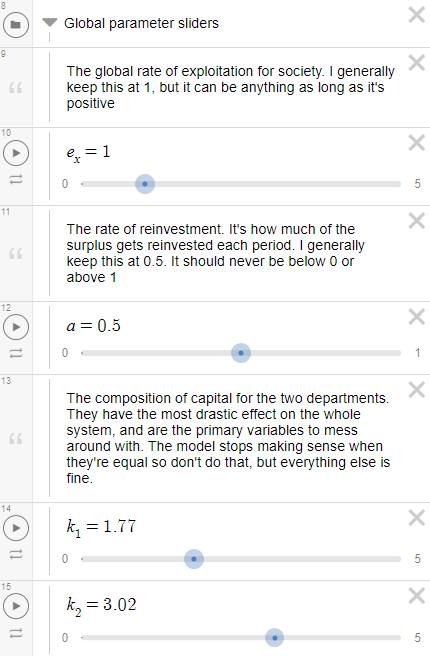
\includegraphics[scale=.7]{Images/globalParameters}
\caption{Open up the global parameters tab to find various numbers which characterize the economy.}
\end{figure}
Also found in this tab are the rate of exploitation $e_x$, which I'll be simply denoting $e$ in this write-up (desmos insists that $e$ by itself is the calculus $e$), and the rate of surplus reinvestment $a$. The rate of exploitation is fixed and assumed constant throughout society. All workers are assumed to be homogeneous in skills and equally exploited. We assume not only that all worker are paid identical amounts for each hour worked but also that they spend these wages consuming the same bundle of goods each period. We'll say more about the variable $a$ in a moment. \par 
An arbitrary hour of value from either department can be broken into two components: value of the raw materials, i.e. dead labor, and value added on top of that, i.e. living labor. The division varies between the departments, but not within them. Thus we have numbers $c_1$, $l_1$, $c_2$ and $l_2$ such that
\begin{align}
	1 = c_1+l_1 = c_2+l_2
\end{align}
Of the living labor, some will have been paid for by the capitalist, while the rest will have been given to them free of charge due to exploitation. Exploitation being a societal constant means that the division of an hour of living labor into `paid time' and `unpaid time' will be the same for both departments. We therefore have the additional numbers $v_1,s_1,v_2$, and $s_2$, so that
\begin{align}
	l_1 = v_1+s_1 \hspace{2cm} l_2 = v_2+s_2
\end{align} 
which satisfy the identity
\begin{align}
	e = \frac{s_1}{v_1} = \frac{s_2}{v_2}
\end{align} 
we can thus replace $s_1$ with $ev_1$ and $s_2$ with $ev_2$ so that
\begin{align}
	l_1 = (1+e)v_1 \hspace{2cm} l_2 = (1+e)v_2 
\end{align} 
Production is broken up into periods. It could be a month, or a year, or whatever. As mentioned earlier, all commodities produced have the same turnover time of exactly one production period.  
\section{Conditions for Growth}
\subsection{Ideal Growth}
What we are interested in tracking with this model is the \textbf{total value output} of the two departments after each period. These are denoted $y_1(t)$ and $y_2(t)$, primarily, where $y_1(4)$ represents the total value output of department 1 at the beginning of the fourth production period. The initial values of these (at time $t=0$) can be set with sliders found in the `Initial conditions sliders' folder.
\begin{figure}[H]
\centering
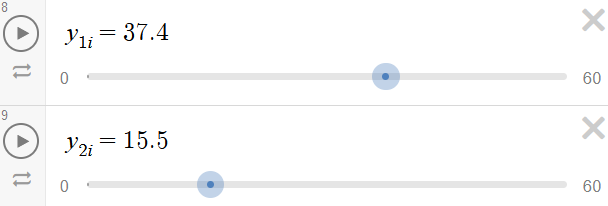
\includegraphics[scale=.5]{Images/initialY}
\caption{Sliders for the initial values of department $1$ and department $2$.}
\end{figure}
As a single hour can be broken uniformly down into living and dead labor, so can the amounts $y_1(t)$ and $y_2(t)$:
\begin{align} 
	& y_1(t) = c_1y_1(t) + l_1y_1(t) \\
	& y_1(t) = c_2y_2(t) + l_2y_2(t) 
\end{align}
since $c_i+v_i = 1_i$ for $i=1,2$. Breaking the $l$ part of these down into a variable and surplus part, we further have 
\begin{align}
	& y_1(t) = c_1y_1(t) + v_1y_1(t) + s_1y_1(t) \\
	& y_1(t) = c_2y_2(t) + v_2y_2(t) + s_2y_2(t)
\end{align} 
Each production period. the capitalists take a fixed, constant percentage of their surplus value and reinvest it into expanding their production, i.e. to accumulating capital. The remainder is consumed. We'll stick to using department $1$ as an example for the moment. Department $1$'s surplus at the end of production period $t$ is $s_1y_1(t)$. $a$ is a number between $0$ and $1$ representing how much of this will be reinvested, while $b=1-a$ is how much will be consumed `unproductively'. The amount being reinvested in department $1$ is therefore 
\begin{align}
	as_1y_1(t) 
\end{align} 
Of this investment, some will be spent on more raw materials while the rest will be spent on additional labor. The division is based on the composition of capital of the department:
\begin{align}
	as_1y_1(t) = \frac{c_1+v_1}{c_2+v_2}as_1y_1(t) = \frac{c_1}{c_1+v_1}as_1y_1(t)+\frac{v_1}{c_1+v_1}as_1y_1(t) 
\end{align} 
(Note that dividing these two quantities by each other gives the composition of capital $k_1$.) Through the magic of exploitation, the variable capital part of this reinvestment will generate additional value output at the end of the next period:
\begin{align}
	\frac{v_1}{c_1+v_1}as_1y_1(t) \to \frac{v_1}{c_1+v_1}as_1y_1(t)+\frac{s_1}{c_1+v_1}as_1y_1(t) 
\end{align} 
The conclusion from this is that given a reinvestment of the amount $as_1y_1(t)$, the output value of department $1$ at the end of the next period will be the old value output plus the reinvestment amount \emph{plus} that extra amount generated by exploitation. I.e.
\begin{align}
	 y_1(t+1) &= y_1(t) + as_1y_1(t) + \frac{s_1}{c_1+v_1}as_1y_1(t) \\
	 		&= y_1(t) + \frac{c_1+v_1}{c_1+v_1}as_1y_1(t) + \frac{s_1}{c_1+v_1}as_1y_1(t) \\
	 		&= y_1(t) + \frac{\cancelto{1}{c_1+v_1+s_1}}{c_1+v_1}as_1y_1(t) \\
	 		&= y_1(t) + \frac{1}{c_1+v_1}as_1y_1(t) \\
	 		&= (1+a\frac{s_1}{c_1+v_1})y_1(t)  \\
	 		&= (1+a\pi_1)y_1(t)
\end{align}
where $\pi_1 = \frac{s_1}{c_1+v_1}$ is the rate of profit for department 1. I.e. each period we get the value by the next period by simply taking the current value and multiply it by $1+\pi_1$. That is to say, given the initial value $y_1(0)$ (represented by $y_{1i}$ in desmos), we have
\begin{align}
	y_1(t) = (1+\frac{as_1}{c_1+v_1})^ty_1(0) \label{dept1Ideal}
\end{align} 
By replacing all of the $1$s with $2$s in the above argument we also have
\begin{align}
	y_2(t) = (1+\frac{as_2}{c_2+v_2})^ty_2(0) \label{dept2Ideal}
\end{align} 
In English these equations say that each production cycle we simply scale up the economy by a percentage fixed by the $c_i,v_i$ and $s_i$. I.e. exponential scaling. The dotted lines represent this ideal growth, and they are the given by the functions $I_1(t)$ and $I_2(t)$ in desmos, found towards the bottom of the 'Growth path of the systems' folder. Graphs of functions can be turned on and off by clicking the circle on their left. Go ahead and turn off everything that is currently turned on, and turn on these functions $I_1$ and $I_2$. You should see something like this:
\begin{figure}[H]
\centering
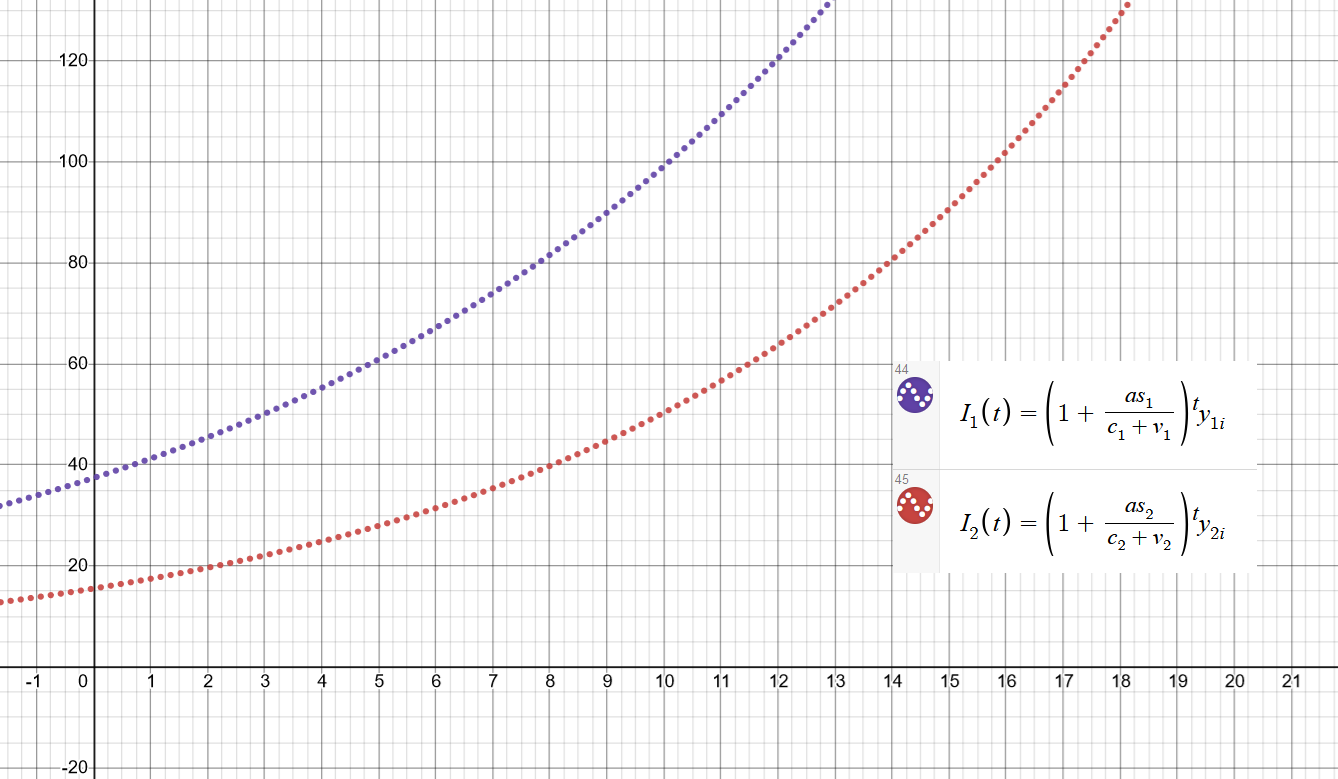
\includegraphics[scale=.5]{Images/dotted}
\caption{The dotted lines represent the growth we would get if capitalists were always able to reinvest exactly how we are assume they want to. (I.e. regardless of what materials are available and regardless of effective demand.)} 
\end{figure}
However, \emph{is this kind of growth even possible}?
\subsection{Warranted Growth}
 Let's consider a concrete example. Suppose $y_1(t) = 100$ and $y_2(t)=100$, $c_1 = v_1 = s_1 = \frac{1}{3}$, $c_2 = \frac{2}{3}$, and $v_2 = s_2 = \frac{1}{6}$. (Note this means that $e = \frac{s_1}{v_1} = \frac{s_2}{v_2} = 1$, $k_1 = 1$ and $k_2 = 4$.) If capitalists were to successfully reinvest in the way we just described, then the output values at time $t+1$ would be
\begin{align}
	& y_1(t+1) = (1+a\frac{s_1}{c_1+v_1})y_1(t) = \left(1+\frac{1}{2}\frac{\frac{1}{3}}{\frac{1}{3}+\frac{1}{3}}\right)100 = \frac{5}{4}(100) = 125 \\
	& y_2(t+1) = (1+\frac{1}{10})100 = \frac{11}{10}(100) = 110
\end{align}
The question we have to ask is: do we have the required materials to do this? Consider the value output of $y_1(t+1) = 125$. This has a constant capital component of $125c_1 \approx 42$. Meanwhile $y_2(t+1) = 110$ has a constant capital component of $110c_2 \approx 74$. Note that constant capital exclusively comes from the capital goods department. Thus the total value of the capital goods department required to produce these outputs from the two departments is around $42+74 = 116 > 100$. Therefore when capitalists go into market intending to purchase the raw materials necessary for production during this period, they will find themselves unable to get everything they need. \par 
Meanwhile variable capital comes exclusively from the wage goods department. $125v_1 \approx 42$ and $110v_2 \approx 18$, so the total variable capital required to produce this output is $42+18=60$. In additional to this requirement, capitalists are going to consume whatever they don't invest, and everything consumed also comes from the wage goods department (which we are assuming includes luxury goods). Thus total amound consumed is $bs_1y_1(t)+bs_2y_2(t) \approx 25$, so the total value of wage goods required to produce these outputs is around $85 < 100$. The wage goods industries thus experience the opposite of what the capital goods industries did: when they bring their goods to market, they will find themselves unable to sell everything. To summarize
\begin{align}
	& c_1y_1(t) + c_2y_2(t) = 114 > y_1(t) \\
	& v_1y_1(t) + v_2y_2(t) + bs_1y_1(t) + bs_2y_2(t) = 85 < 100
\end{align}
Growth along the ideal paths we plotted above is therefore \emph{impossible}. There are not enough capital goods, not to mention too many wage goods (if equilibrium is to be maintained, this will not do either). \par 
This is where Marx got stuck when writing volume 2 of Capital. In chapter 21 of that book, he begins with the reasonable assumption that \emph{both} departments accumulate half of their surplus value. However, he doesn't proceed with this assumption. Instead he has the capitalists in department 1 reinvesting half of their surplus value, while capitalists in department 2 reinvest \emph{as much or as little} of their surplus as is necessary to facilitate the accumulation of department 1. We will see that generally this has capitalists in department 2 reinvesting at a completely different rate from those of department 1. \par 
Marx clearly lacked the mathematical tools that he needed to do what he originally wanted to with his reproduction schema. However, we do not. We thus proceed with his original idea: each period, a certain percentage of the total surplus is consumed each period, given by $b=1-a$. The rest of the surplus is reinvested in production. The goal is to figure out how this can be done while maintaining consistent supply-demand equilibrium. \par 
A fairly startling realization that we come to immediately when we start to consider accomplishing this task is that it likely has to involve \emph{downsizing} the wage goods department, rather than expanding it. We just noted that we'll have an oversupply of them if we try to accumulate equally. More importantly, the labor goods department (I'll use this interchangeably with the wage goods department) \emph{has a higher composition of capital than the capital goods department}. This means that to accumulate at all in this department requires far more capital goods than accumulation in the capital goods department, and we just noted that in the `ideal' conditions of accumulation we have an undersupply of capital goods. In other words, and capitalists that were previously invested entirely in department 2 that want to accumulate the same amount of capital as all the other capitalists will be forced to diversify, and shift their existing capital from department 2 into department 1. \par 
In fact, it turns out that there is only ever a single way to accomplish the task Marx originally wanted to model. Indeed, that way is to not only invest \emph{all} of the total surplus into the capital goods department, but also to halve the size of the wage goods department. Specifically, if we consider $y_1(t+1) = 200$ and $y_2(t+1) = 45$, then indeed we have
\begin{align}
	c_1(200) + c_2(45) = 100 \\
	v_1(200)+v_2(45)+bs_1(100)+bs_2(100) = 100
\end{align} 
I.e. this scaling perfectly uses up the $100$ units of value in capital goods and the $100$ units in wage goods, while allocating $b\times 100$ percent of the surplus to capitalist consumption. But now let us consider the task of accumulating the same percentage of surplus for the next period. We find ourselves with the same problem as before, but reversed, and more dramatic. To just scale up the capital goods industry alone by $a \times 100$ percent of it's surplus would require $70$ units of variable capital, and we only have $45$ to begin with! Again we are faced with the requirement of massively downscaling the capital goods department and investing all of the reinvestment fund into the wage goods department. And back and forth we go. Except we don't, because at this point there is no way to shift around capital in order to reinvest the surplus and use up all of the produce. I mentioned that there is always exactly one pair of numbers for $y_1(t+2)$ and $y_2(t+2)$ which satisfied the conditions we imposed. But this time those numbers are $y_2(t+2) \approx 409$, and $y_1(t) \approx -184$. We get a negative result in the capital goods department, which is nonsensical. \par
It should be kept in mind that each time capital is taken out of one industry and put into another, workers in the former industry are laid off. This of course also creates jobs in the other industry which could potentially employ those laid off workers, but this likely requires them to relocate and completely rearrange their lives. Even if they find new jobs immediately, this process will be massively disruptive to broad swathes of the workforce. Moreover, if capital shifts in it's biases from less capital intensive industries into more capital intensive industries, i.e. industries with higher compositions of capital, then there won't be enough new job openings to hire the workers that were laid off. In other words, half of the time this happens, large numbers of workers won't be able to find new jobs at all, and go hungry. \par 
To analyze the situation further we need to finally state the problem formally. In order to analyze effectively what equilibrium growth looks like in a naturally accumulating capitalist economy, we have to solve is the system of equations
\begin{align}
	& y_1(t) = c_1y_1(t+1) + c_2y_2(t+1) \label{sys1} \\
	& y_2(t) = v_1y_1(t+1) + v_2y_2(t+1) + bs_1y_1(t) + bs_2y_2(t) \label{sys2}
\end{align}
To repeat these requirements in English, we are seeking growth paths $y_1$ and $y_2$ such that at the end of each production period, we have exactly what is necessary to produce the next periods output, while also leaving enough aside for the capitalists to consume the proportion $b$ of their surplus. The central condition that the total capital accumulated is $a$ times the total surplus value is here, i.e. that
\[ (c_1+v_1)y_1+(c_2+v_2)y_2=a(s_1y_1+s_2y_2) \]
is implied by these equations. See appendix \ref{appendixA} beginning at equation \ref{surplusEquation} for a derivation of this. \par 
Even if Marx had been able to write these equations down, he would not have been able to solve them. What we have here is a system of difference equations. Note that the variable here being solved for is a pair of \emph{function}, i.e. curves, rather than numbers. For those who really want to see it, the process of solving this can be found in appendix B. However, it's better seen visually, which is the purpose of this guide. \par 
We're going to call the solutions to these \textbf{warranted} growth paths. They are labeled $y_1(t)$ and $y_2(t)$ in Desmos. Go ahead and turn them on now. For all functions which have two definitions, you should either keep both turned on or both turned off.
\begin{figure}[H] 
\centering
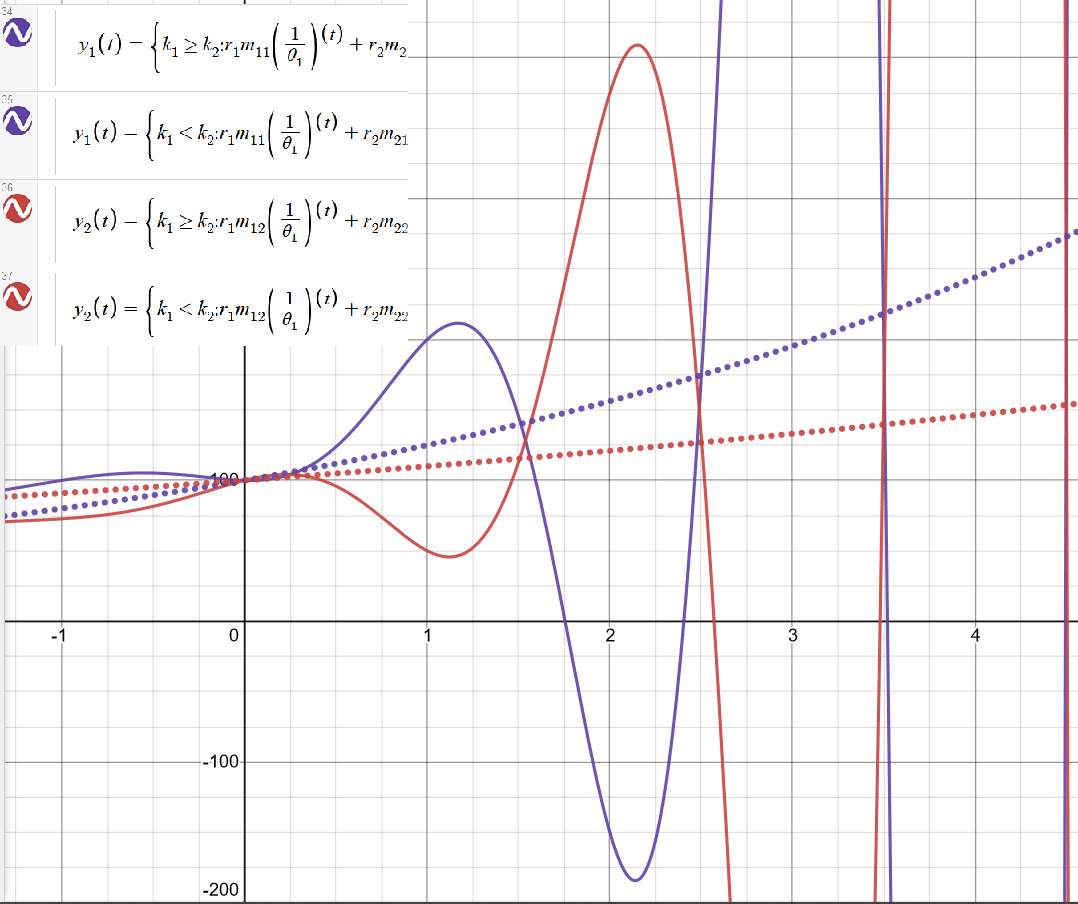
\includegraphics[scale=.5]{Images/conditionsP}
\caption{Solid lines a path in which conditions for reinvestment are consistently met.} 
\label{fig:contradiction}
\end{figure}
If you haven't changed anything then the curves your looking at are exactly what we've been using for this example. You can confirm this by noting that $y_1(0)$ and $y_2(0)$ are set to $100$ and noting that the values at $t=1$ and $t=2$ are exactly what I said they were. It needs to be emphasized that the solid lines are the \emph{only} way in which the economy can grow and meet the requirements we've imposed. In other words, since both curves routinely dip into negative values which are meaningless within our model, it literally can't, at least not indefinitely. \par 
\subsection{The Crisis of Disproportionality}
These curves only indicate \emph{how} the conditions might be met. But will they? Why should the capitalist class act in such a way as to follow these warranted paths? Well, yes and no. We'll address the no part first. \par 
In capital volume 2, Marx breaks the circulatory system of capitalism down into three subcirculations. First, there are the two \emph{intra}departmental circulations. In department 1, this is the circulation of means of production which are being used to produce more means of production. We'll call this circulation 1. In department 2, this is the circulation of consumer goods being consumed by capitalists and workers in department 2. We'll call this circulation 2. Finally, we have the interdepartmental circulation between the two departments. We'll call this circulation 3. \par 
All three of these circulations have unique qualities and potentials for producing crisis and disruption. Circulation 1, for example, is where we find all of the supply chains that we're all becoming so familiar with. Supply chain breakdowns are therefore a crisis characteristic of circulation 1. Meanwhile, overproduction/underconsumption crises are what we find when we look closely at department 2, since that circulation has the workers themselves purchasing and consuming the product as a critical moment. \par 
The growth paths we've derived have assume no issues are put up by circulations 1 or 2. Is this reasonable? Of course not. Overproduction is endemic to capitalism itself, and our supply chains have over time become increasingly fragile and vulnerable to external shocks due to the system's aversion to idle capital (hence organizational technologies like just-in-time production). Let's nonetheless suppose that these problems are not present. At that point, we can say that these growth paths are warranted \emph{to the extent} that capitalists maintain supply-demand equilibrium and grow in the way that they naturally want to. The political economists of Marx's time believed that `if only' conditions were perfect, that the accumulation of capital would resolve into a utopian and peaceful world. The true impact of these explosive growth curves is that they reveal how false that claim truly is. \par 
What we are showing with these curves is that a world in which capitalists were free to reinvest as they saw fit with no external restrictions aside from the goods available for expansion being limited to what the capitalists have produced previously would be subject to routine, cascading, massive disruptions and chaos. In other words, it would produce it's own crises; crises of \emph{disproportionality}.  \par
Many Marxists mistake crises of disproportionality for crises of overproduction. Of course, all crises which receive that label are, to some extent, crises of overproduction. But overproduction within capitalism happens for two reasons. One reason is the contradiction between increasing exploitation of the general population and increasing productivity and output. In other words, a lack of buying power on the part of workers. However, another reason, always equally implicit to any such crisis, is the investment decisions of the capitalist class. Too much of this, too little of that. These curves, which Marx would have derived if he had the mathematical tools available to him, show that this phenomena of disproportionality is as endemic to capitalism as that of denying the consumer their ability to consume. \par 
This distinction is important, because a true, \emph{pure} crisis of overproduction is a much deeper crisis for capitalism than the periodically occurring crisis of disproportionality. In my opinion, there have only ever been two of these. The first was in 1914. By that point, the world had been fully carved up by the European capitalist powers. Until then, periodic disproportions aside, colonization of the new world and imperialism created constantly expanding consumer markets. As long as these processes existed, capitalists were free to exploit their workers more and more without fear of losing their ability to sell their products. In 1914, there was no more room to expand, and the system spiraled into chaos. The 31 years between 1914 and 1945 should be seen as a singular crisis of overproduction, in which capitalism struggled and repeatedly failed to reconfigure itself to create a steady supply of demand. \par 
The new supply of demand which was finally created by 1945 came from the only place that it could have: the workers of Europe themselves. The capitalist class is \emph{incapable} of fixing a pure crisis of overproduction. Their basic incentive structures prevent them from raising wages to allow their workers more buying power. Only significant threat from the workers themselves could facilitate such a massive systemic shift. True crises of overproduction are apocalyptic events. They don't just come and get patched up like the crises of other sorts. War is the only way out. Class wars, world wars, you name it. Moreover, such a systemic shift in the system can only be enforced by a political distribution in which some power is shared with the working class. \par 
However, when workers have the power to demand higher wages, which is precisely what they had to have taken for themselves to solve the crisis of overproduction, they are going to press that demand as far as they can. And so they did, until capitalism hit a rate of profit crisis. What followed was the capitalists quietly re-seizing power and instituting neoliberalism. Labor was disciplined and their buying power began to be reduced again. The situation was masked by credit bubbles, which finally popped in 2008. That crisis never ended. We currently facing the second true crisis of overproduction in the history of capitalism. \par 
\subsection{Why do the curves look like this?}
What we are therefore observing our model is a capitalist system in which the crisis of disproportionality is the only kind of crisis that the system experiences. There is no overproduction. It is essential to understand this when attempting to understand why these curves look the way they do. These growth paths maintain \emph{perpetual} supply-demand equilibrium. That is what they exist to do. Thus we cannot explain why these crises arise in terms of capitalists following price signals. To follow price signals is to adjust production according to prices rising and falling, but supply-demand equilibrium means that prices remain the same at all times. There has to be some other reason why capitalists are destined to follow these paths. \par 
The reason why these paths look the way they do has everything to do with the differing compositions of capital between the two departments. In the current case we are looking at, the labor goods department has a higher composition than the capital goods department. A higher composition means higher capital intensity. A fixed amount of capital invested in department 2 requires more capital goods than an equal investment in department 1. What we need to note is the inward facing dependency implicit to this setup. The labor goods department is overly dependent on the capital goods department, while the capital goods department is overly dependent on the labor goods department. Hence the sloshing back and forth. \par 
However, growth paths of the oscillatory type we've been observing only occur when $k_2 > k_1$. When $k_2 < k_1$, we get very different looking growth paths. Right now, it should be set so that $k_1=1$ and $k_2=4$. Go ahead and change $k_1$ to equal $2$ and $k_1=1$ to see the second type of growth. 
\begin{figure}[H] 
\centering
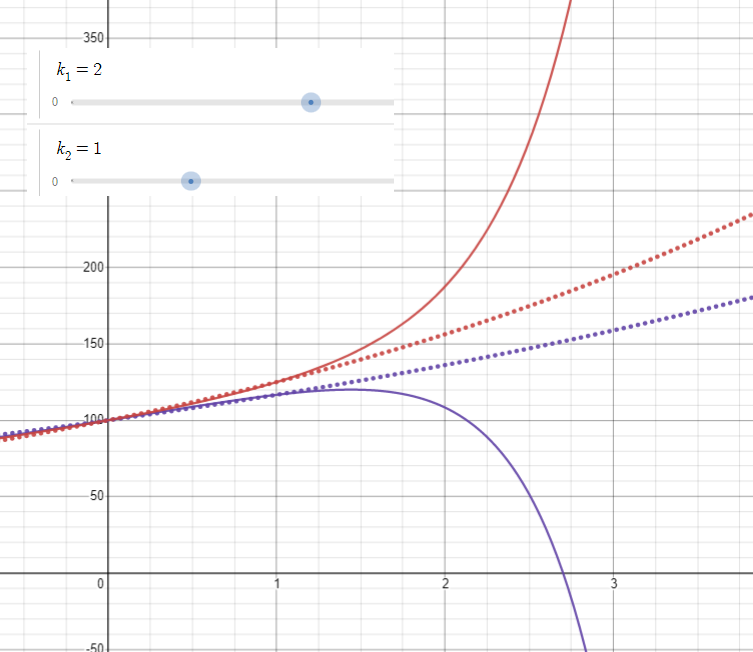
\includegraphics[scale=.5]{Images/monotonicG}
\caption{When $k_1 > k_2$, we lose oscillation and instead get growth in which the two departments monotonically diverge from each other.} 
\end{figure}
First of all, let's note that the during the first period, the capitalist class might be forgiven for thinking that their individual decisions to reinvest might produce stable, balanced growth! The warranted growth paths seem identical to the ideal growth paths that we started with. At the end of the first period, we are faced with a similar problem to before; the natural capitalist growth is impossible given the available output from the two departments. At this point we see the capitalists start to desert the capital goods department entirely. Unlike the situation when $k_2 < k_1$, we don't get a swing in the other direction. Things simply continue in that direction until the capital goods department stops existing. \par 
How could it get to this point? Again, let us consider the compositions of capital. With $k_2 < k_1$, we have a capital goods department which is overdependent on capital goods, and a labor goods department which is overdependent on labor goods. In other words, each department is overdependent on \emph{itself}. We go from an inward facing dependency to an outward facing one, and the growth paths reflect this. That is the basic intuitive reason why these curves look the way they do. Disproportions arise due to technological asymmetry. \par 
The reader who feels satisfied by that explanation should feel free to move on to the next section now. The rest of this section is dedicated to understanding the matter in more detail. Now, as we mentioned, constant supply-demand equilibrium means we never have explicit oversupply or undersupply of anything. However, it is helpful to talk in terms of this anyway. In the next section we will discuss balanced growth, and with a simple finding and replacing from `over/undersupply' of disproportionalities over or under the balanced growth paths, the following discussion can be reworded to something more technically correct. Suppose we have an oversupply of capital goods and an undersupply of wage goods. Can the capitalists help themselves here? The warranted growth path seems to believe that they can't but let's think through it ourselves. Capitalists would need to shift capital away from the more capital intensive industries towards the more labor intensive one. This move would shift society into being more labor intensive generally, and therefore it would require a more intensive usage of wage goods. This isn't exactly easy when there is currently an undersupply of wage goods. Furthermore, it requires a less intensive use of capital goods, which there is currently an undersupply of. One can see then the difficulties implicit to addressing the problem. They seem to require that the problem not be there in the first place! This is why we see in the growth paths a society which simply doubles down, becoming more and more focused on making capital goods and less and less focused on making wage goods over time. An identical argument can be made in the case where there is an initial undersupply of capital goods and oversupply of wage goods. \par 
Let's return to the case $k_2 > k_1$. Suppose this is the case, and we have an oversupply of capital goods and an undersupply of wage goods. The solution then would be to shift away the capital goods industry, which is less capital intensive, and towards the wage goods industry, which is more capital intensive. Thus to address the problem involves making a more overall capital intensive society, and less labor intensive. This means that addressing an oversupply/undersupply problem not only is possible, unlike the case where $k_2 < k_1$, but it is very likely to \emph{overcompensate}, because it more rapidly consumes what there is an oversupply of and less rapidly consumes what there is an undersupply of. The same thing happens when there is an oversupply of wage goods and an undersupply of wage goods. The two departments end up flying by each other repeatedly, hence the oscillation. \par 
To summarize, there is a contradiction between the capitalists need to shift their capital between different departments, and the differing compositions of capital of those departments. This contradiction spins capitalism into periodic disproportionality crises during it's natural course of accumulation. \par 
It is finally worth re-emphasizing that these warranted paths diverge from reality at the point when the curves go negative. There would have been a crisis, and a subsequent break in continuity, before this happens. We know what happens at the point of a crisis: either a revolutionary overthrow of capitalism, or more important to our analysis, \emph{a break in continuity}, in which some central apparatus; likely a state along with top financial institutions, inevitably steps in to \emph{reset} things back to something approximating balanced growth, which is what we're about to talk about.  \par  
  In general, we're going to see the economy go through one minor earthquake, and then something which appears more as a crisis, followed finally nothing which has any meaning in our reality. Our interpretation is going to be that each crisis resets us to some new graph of these curves at time $t=0$, with initial conditions which buy the capitalist system a few more periods of stable growth. The next question we need to ask then, is the following: will they ever actually \emph{find} some kind of stable growth? Or are these crises simply bound to repeat themselves over and over?
\section{The Search for Stability}
First, some housekeeping. Go ahead and turn off the ideal growth paths $I_1(t)$ and $I_2(t)$ if you had them on. Now that we've confirmed that the warranted growth paths are what we are likely to get instead, we won't have much need of them for the rest of this guide. Next, click one of the numbers on either side of the sliders for $y_{1i}$ and $y_{2i}$ to edit their ranges. We're going to bring things way down so that our growth curves can generally appear on the same screen as our other variables, which tend to be proportions and as such tend to be quite small. I'd recommend having the min be $0$ and the max be something like $10$, with a very small step size:
\begin{figure}[H]
\centering
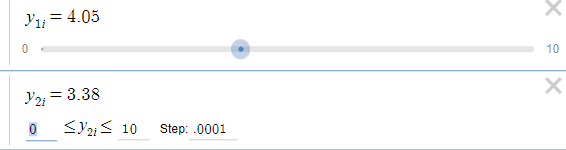
\includegraphics[scale=0.7]{Images/bringingItDOwn}
\end{figure}
 To accompany this we need to change the range of the $y$ axis. Click the wrench icon at the top right of the screen. Here you can change the bounds for the two axes. I recommend for our purposes having the $x$-axis start very slightly negative and go no farther than 9 or 10, while doing something similar for $y$. 
\begin{figure}[H]
\centering
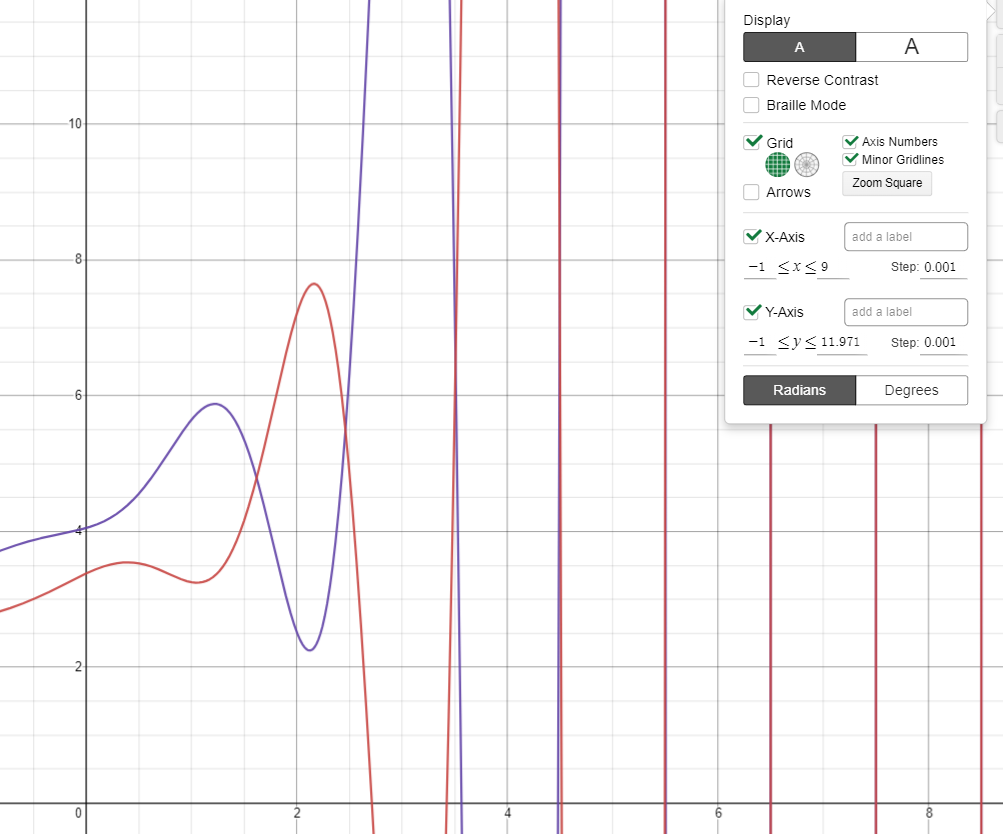
\includegraphics[scale=0.5]{Images/wrench}
\end{figure}
As you can see I've also altered the compositions of capital to make $k_2 > k_1$. Those paths will be our default because oscillations are fun. I recommend a very small step size for the $k$'s and don't think there is much need for them to range much higher than $5$ or $6$. \par 
Once that's all taken care of, go ahead and turn on the two functions $z_{g1}$ and $z_{g2}$, located directly below the $y_1$ and $y_2$ functions. I recommend keeping these turned on whenever you have the $y_i(t)$'s themselves turned on for the rest of the guide. My initial conditions and compositions of capital are also displayed so you can copy them if you want to follow along. 
\begin{figure}[H]
\centering
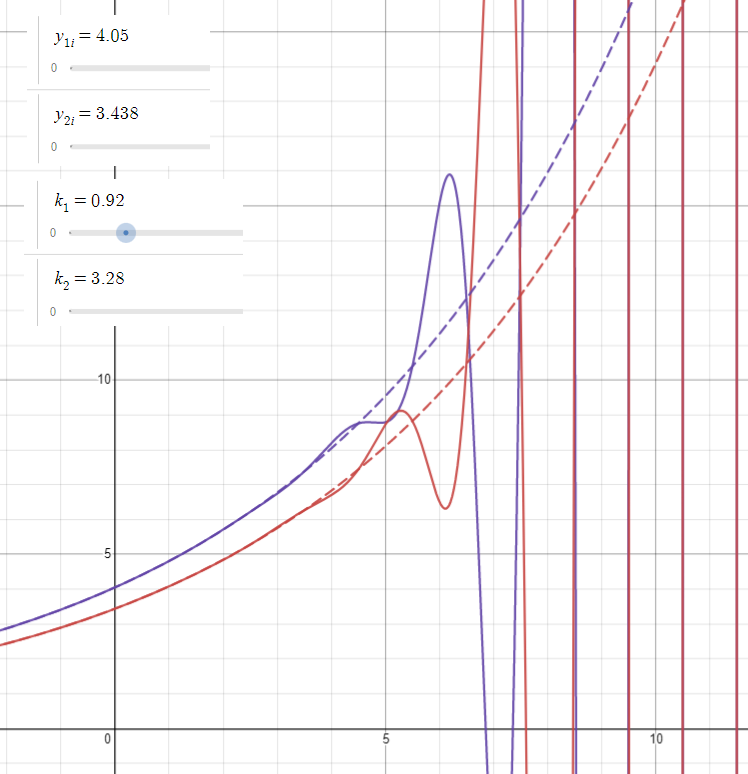
\includegraphics[scale=0.7]{Images/balancedPaths}
\label{fig:balancedGrowth}
\caption{Based on how close to the initial conditions we are, the $y_1(t)$ and $y_2(t)$ follow the equilibrium paths for a few productive cycles, then fly off of them suddenly and violently.} 
\end{figure}
The significance of this \textbf{balanced growth path} is that for the current value of $y_{1i}$, these are the \emph{only} paths in which both departments stay positive, \emph{let alone} achieve any kind of harmonious growth. I can't stress that enough. If the capitalists desire prosperity, then these paths are their \emph{only} option. The security of the system therefore depends on their ability to get close to one of these special paths in the aftermath of a crisis. What we are interested in evaluating is how easy of a time they are going to have staying on it. \par 
 Scroll back up to the $y_{1i}$ and $y_{2i}$ sliders. For any choice of $y_{1i}$, there is a single associated $y_{2i}$ which produces this kind of growth. You can see that in our current case, growth progresses \emph{along} the balanced growth path, and then becomes unstable and is violently flung off of it. Why did this happen? Zoom in on $t=0$. Specifically at the red curves.
\begin{figure}[H] 
\centering
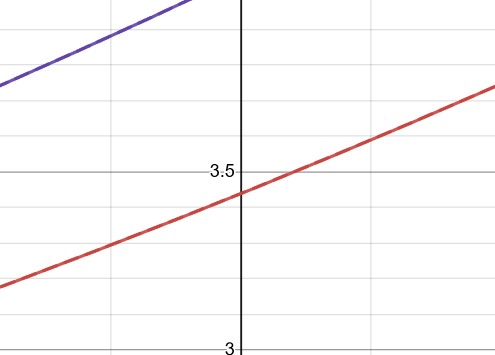
\includegraphics[scale=0.8]{Images/close} 
\end{figure}
Closer...
\begin{figure}[H] 
\centering
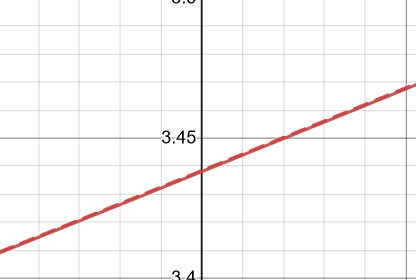
\includegraphics[scale=1]{Images/close1} 
\end{figure}
Closer...........
\begin{figure}[H] 
\centering
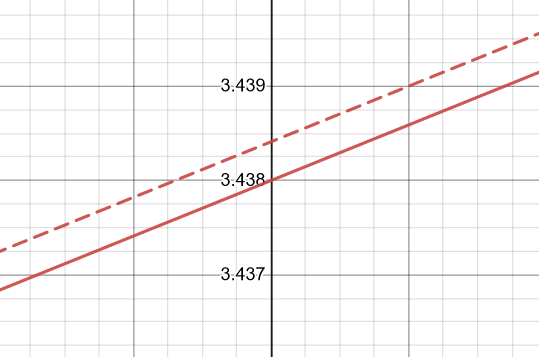
\includegraphics[scale=0.9]{Images/close2} 
\end{figure}
Aha! Our initial conditions were off. $y_{2i}$ was off by uh... about one ten thousandth of a percent. That's it. Just that was enough to cause the economy to spiral into oblivion in less than 5 cycles. You might have noticed that the initial position for $y_1$ is seen as perfect, with all of the `blame' placed on the consumer goods department. In order to have balanced growth paths displaying and moving along with the warranted curves, I had to fix one of the initial conditions to always be perfect, because otherwise it would be ambiguous what to display. The idea is that you can move around the slider for $y_{1i}$, and the balanced path moves with it, while the wage goods curves will diverge from each other. You can then approach balanced growth by using the $y_{2i}$ slider to bring the solid red curve up or down to wherever the dashed curve is. 
 \begin{figure}[H]
\centering
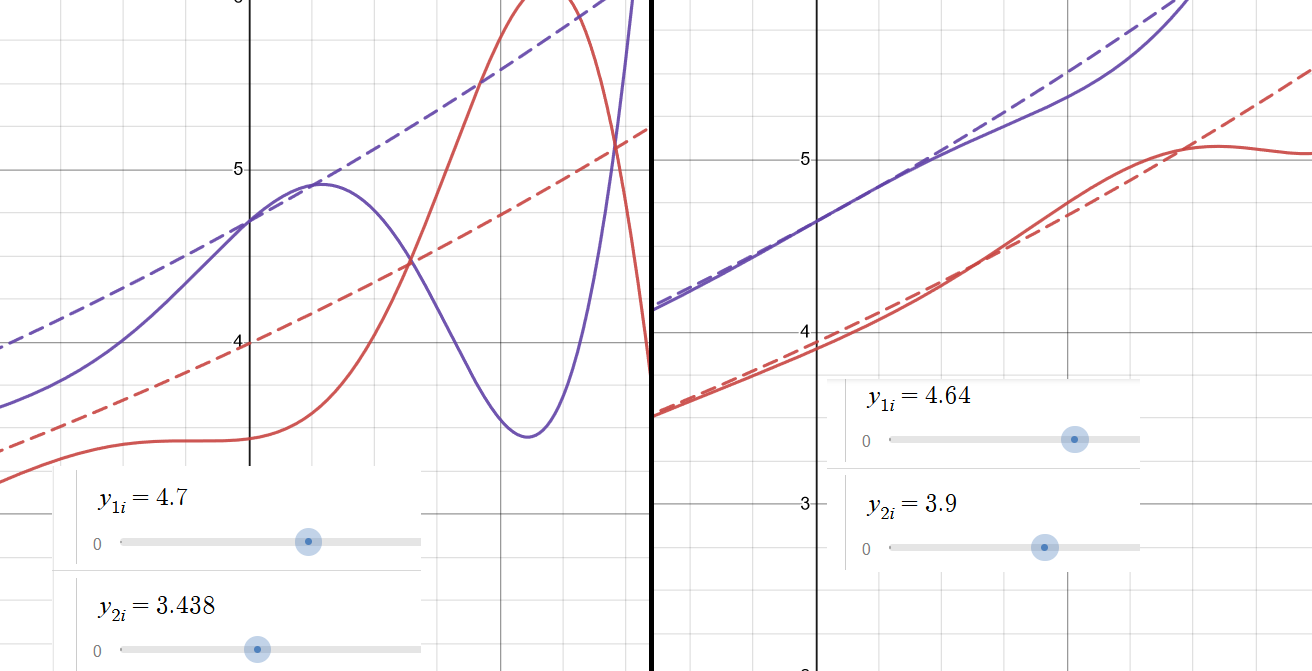
\includegraphics[scale=.6]{Images/liningUp}
\caption{User guide: Move the $y_{1i}$ slider first to wherever you want it, \emph{then} move the $y_{2i}$ slider with the goal of taking the solid red curve to meet the dashed one, in order to approached balanced growth.}
\end{figure}
The numbers beneath these sliders give you the exact values that $y_{1i}$ and $y_{2i}$ need two be in order to achieve balanced growth (in that order). Sliding the red curve in line with the dashed curve amounts to sliding it towards the number $b_{g2}$.
\begin{figure}[H]
\centering
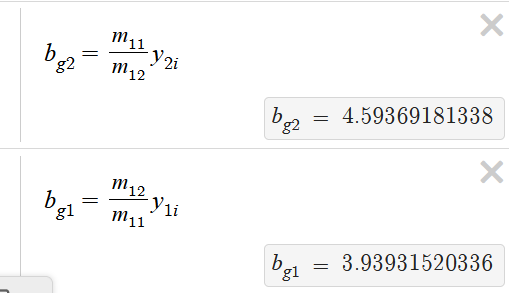
\includegraphics[scale=.7]{Images/initSliders}
\caption{You can see here that the number we were moving $y_{2i}$ towards in the previous figure is $b_{g1}$}
\end{figure}
$b_{g2}$ never actually changes because of the way I've sort of wired this thing with bias towards $y_{1i}$. It wasn't always like this, though. An alternative to this method of displaying balanced growth paths is provided which is technically a tiny bit wrong, but also I think a lot nicer to deal with. Hit up the `Growth paths of the system' folder again. Go ahead and turn off the $z_{g1}$ and $z_{g2}$ functions, and turn on the \emph{almost} balanced growth paths $z_{l1}$ and $z_{l2}$ (the l stands for lie). \par 
\begin{figure}[H]
\centering
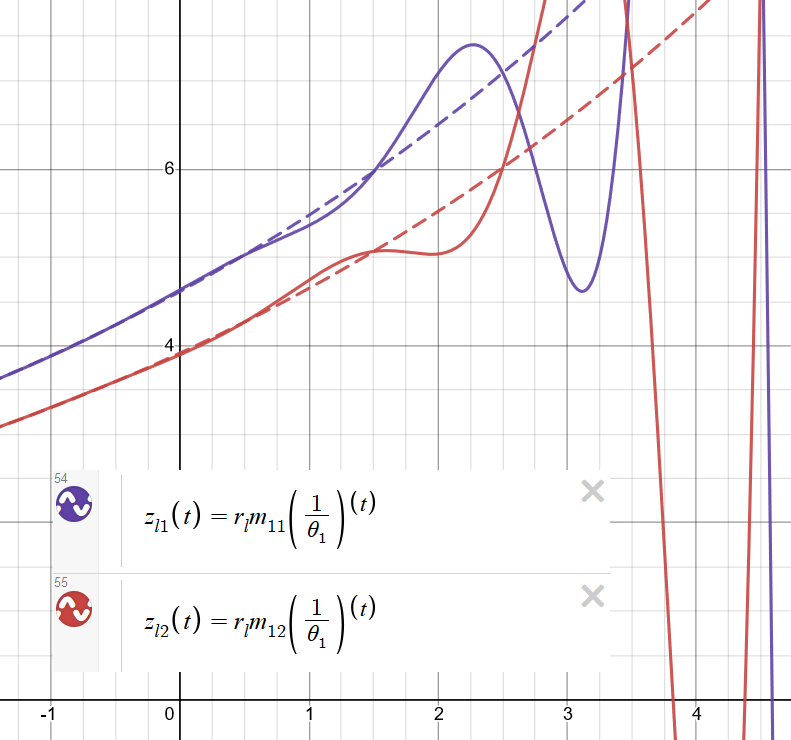
\includegraphics[scale=.7]{Images/almostBalancedGrowth}
\caption{These are technically wrong but also probably better.}
\end{figure}
You can see now by moving around the $y_{1i}$ and $y_{2i}$ sliders that $y_{1i}$ is no longer always perfect. Instead, both departments are blamed equally for any disproportions (the blame is averaged). I think this looks nicer and also makes it easier to configure interesting systems. The trade off, of course, is that these aren't ever \emph{actually} balanced growth paths. However, they \emph{do} become balanced growth paths when $y_{1i}$ and $y_{2i}$ are perfectly aligned. Moreover they are generally extremely close to balanced growth paths, to the point where I didn't even noticed that they weren't until writing section $4$ of this guide. Because of that, I am going to use these functions instead of the actual functions $z_{g1}$ and $z_{g2}$ until we get to that section. Until then, you have my word that using these instead of the more accurate functions won't produce any significant misconceptions. \par 
\begin{figure}[H]
\centering
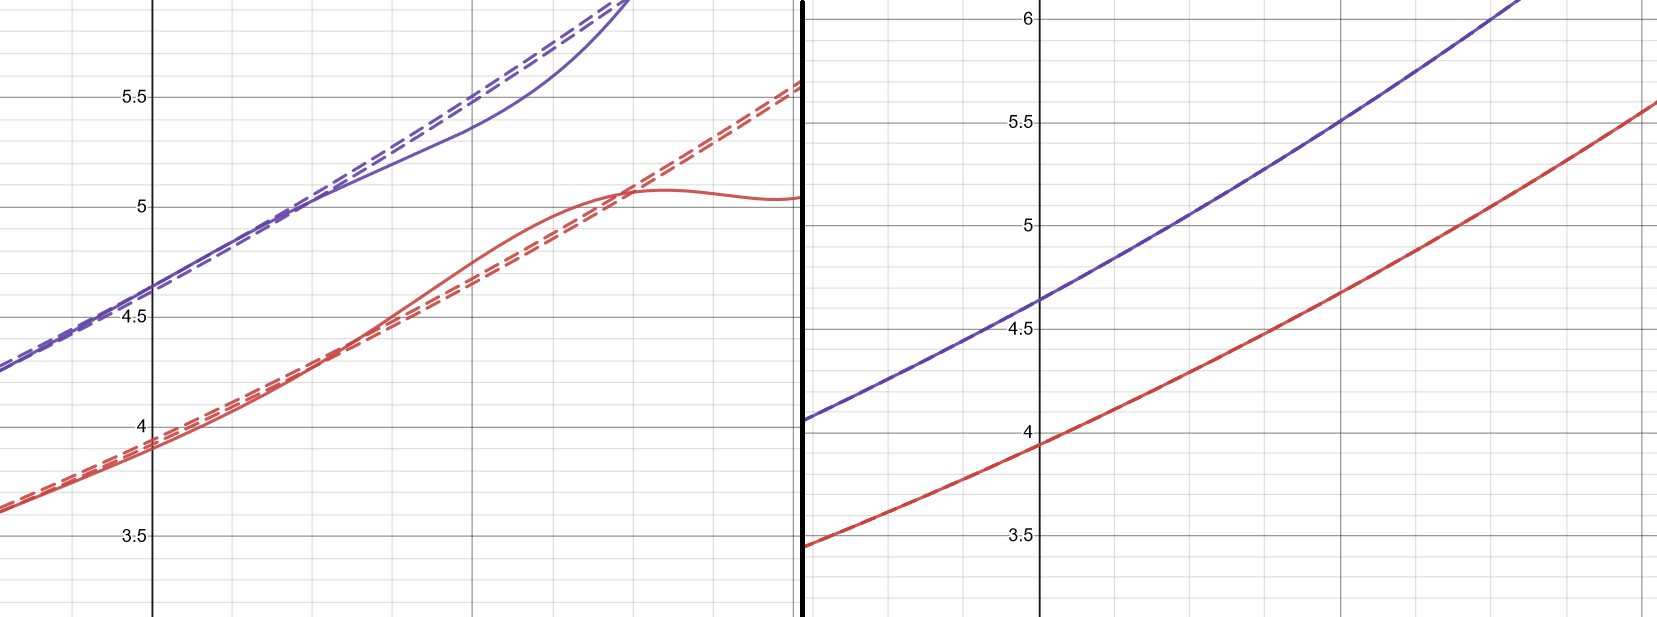
\includegraphics[scale=.5]{Images/verySimilar}
\caption{You can see how close the almost balanced growth paths are to the actual ones here. As $y_1$ and $y_2$ approach actual balanced growth, the difference vanishes.}
\end{figure}
As we mentioned earlier, we can expect that every time capitalism enters a crisis and isn't overthrown, the managers of the system will \emph{reset} the system closer to balanced growth. This is accomplished by the destruction of a significant amount of the capital. If they do a really, really good job of this, they'll have something similar to the settings of my figure \ref{fig:balancedGrowth}. Two things should immediately be noted about a capitalist system set loose with these settings.\par 
First, nobody living in the system will see any sign that things aren't perfect until right before period $5$. The instability doesn't set in gradually. It sets in suddenly, and violently, with very little time to react. This suddenness of the disproportions has ideological consequences. It means that within our system, capitalists will have four production cycles in which they can convince themselves that everything is fine, and that market forces \emph{can} coordinate a stably growing economy after all. In other words, the fact that instability is so sudden is likely to create a false sense of confidence among the people inside of it. It encourages people experiencing crises to focus on proximate causes, such as pandemics and wars, rather than the market forces which are driving things on a more basic level.  \par
Second, the system gets three oscillations before entering total collapse. The first one, beginning around period $4$, is likely perceived as minor earthquake, nothing too serious. The second, occurring at the start of period $5$, is a `natural' disaster. The third, at period $6$, is likely the crisis itself. We'll see as we go that this isn't unique to this system. We always tend to get one or two shake-ups, then a crisis. Those numbers won't change much. \par 
We can confirm this as we revisit the question of how easily capitalists will achieve \emph{true} stability. Obviously the capitalists would appreciate more than just $5$ cycles of steady growth. Let's see how much more we can give them by adding more of the digits of $b_{g1}$ to $y_{2i}$. 
\begin{figure}[H]
\centering
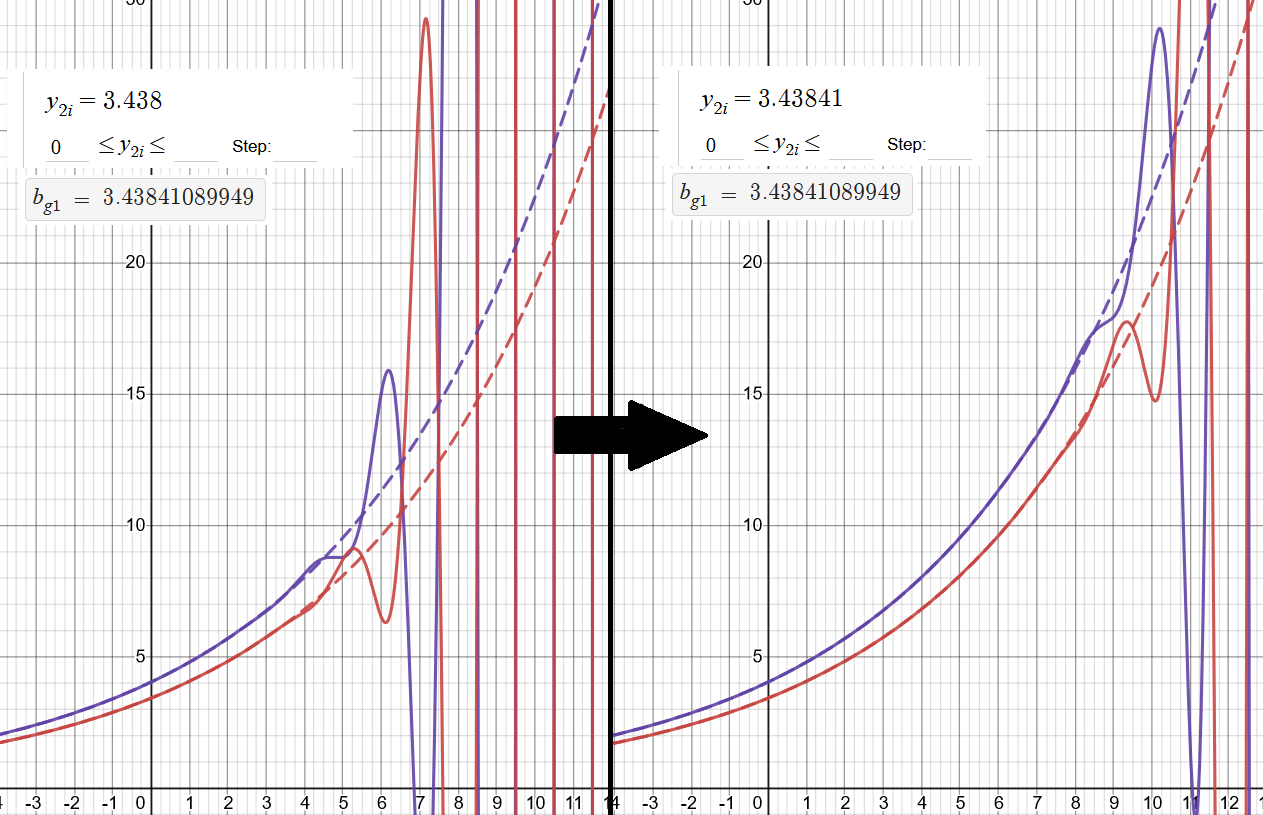
\includegraphics[scale=.6]{Images/approachingEQ}
\caption{Sliding $y_{2i}$ closer to $b_{g1}$ will make the solid line (actual growth) stay matching with the dashed line (balanced growth) before blasting away from it.}
\end{figure} 
However, you'll notice that it's very hard to fully achieve equilibrium. You can do a bit better for yourself by clicking one of the numbers on either side of the slider, and setting it to be between two numbers which are very close to $b_{g1}$, with a very small step size:
\begin{figure}[H]
\centering
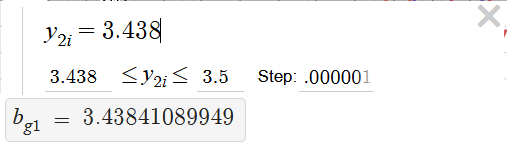
\includegraphics[scale=1]{Images/morePrecision}
\caption{Setting the bounds of the slider so that I can approach \emph{very very close} to $b_{g1}$.}
\end{figure} 
However even if we literally copy and paste the number in, we \emph{still} won't achieve balanced growth!
\begin{figure}[H]
\centering
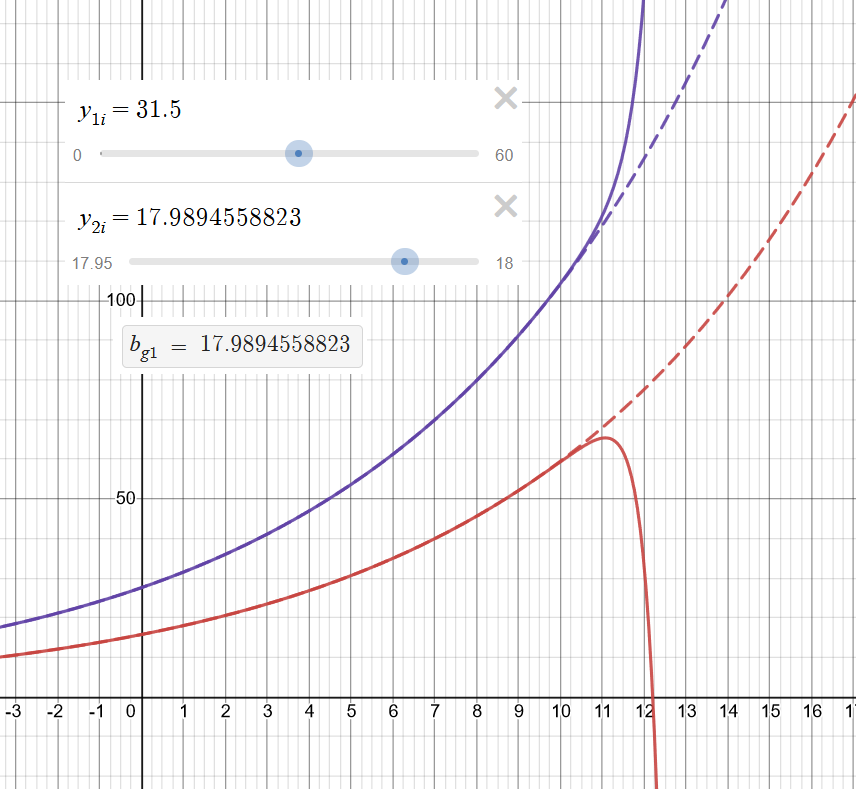
\includegraphics[scale=0.7]{Images/stillMorePrecision}
\caption{\emph{Still} blows up!}
\end{figure} 
The only way to get the systems to actually match up is to simply equate the numbers symbolically:
\begin{figure}[H]
\centering
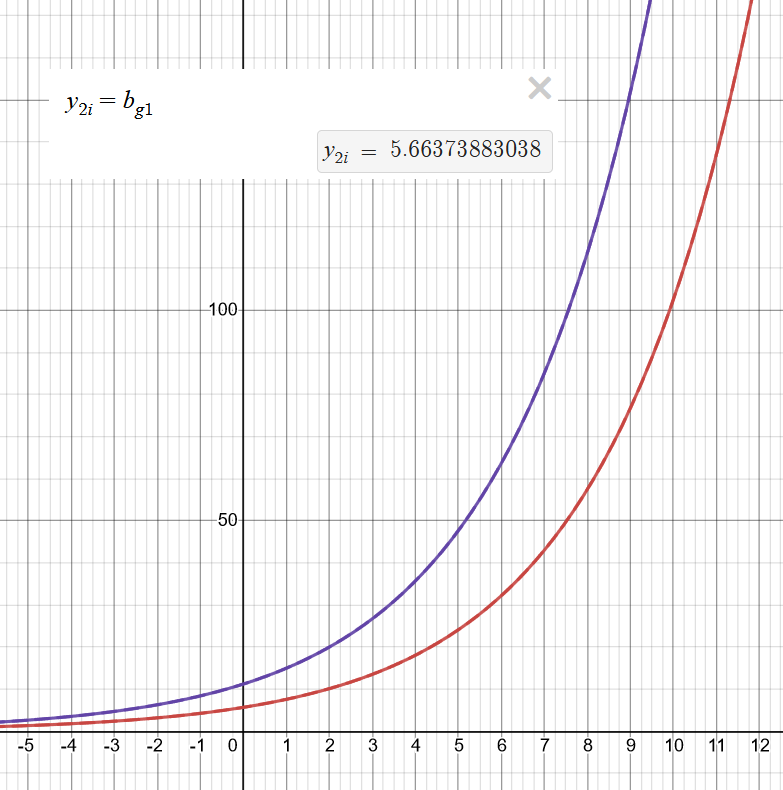
\includegraphics[scale=0.7]{Images/trulyBalanced}
\caption{Copy paste the \emph{letters} rather than the number, and you'll achieve true balanced growth.}
\end{figure} 
Leaving these symbolically equated will allow us to manipulate other parameters of our system and \emph{stay} in balanced growth, which will be helpful later. To go back to a slider for $y_{2i}$ after symbolically setting it to $b_{g1}$, simply delete the symbol you've equated to it and write in any number, then hit enter. The slider will reappear. We'll be making a lot of use of balanced growth analysis, so make sure you're able to go back and forth like this before continuing. \par 

What we've been observing is the significance of the fact that the balanced growth path is \emph{unstable}. Our warranted paths follow them and then suddenly and violently blast away. Moreover the system is \emph{extremely chaotic}. Even a few hundred thousandths of a percent difference can significantly alter the trajectory of the economy. Even if the capitalists manage to set the initial conditions perfectly up to 11 significant figures, they'll still be lucky to get more than a dozen cycles of balanced growth before facing a crisis. \par 
Within the volumes of capital, Marx is seeking to critique the political economists of his time by evaluating their ideal system on their own terms. What this model demonstrates is that their ideal equilibrium can't be expected to produce balanced growth, as they believed. In fact, the instability of ideal growth paths means that capitalists will \emph{never} find themselves on a truly balanced growth path. After a crisis, the likelihood that the capitalist class will manage to initialize it's system in absolutely perfect conditions for balanced growth is the same likelihood that I spontaneously combust while typing this sentence. It's not even worth considering. \par 
This is the conclusion Marx was trying to arrive at with his reproduction schema. But what we've been left with is a model within which we can evaluate all manner of other Marxist concepts and arguments. To facilitate this I've added a bunch of neat functions displaying variables we'd want to track. Let's begin going through those.
\section{Accumulation and the Reserve Army}
\subsection{Net Output in Labor Time}
Scroll down below the functions we've discussed already to find a folder titled `other functions related to the system', and open it up if it isn't already. We'll go through these functions one at a time. The first one we have is net output of society in terms of labor time. It is the function:
\[ Y(t) = y_2(t)+y_1(t)-(c_1y_1(t)+c_2y_2(t)) \]
Note that along the balanced growth path, $c_1y_1(t) + c_2y_2(t) = y_1(t-1)$, i.e. it is the constant capital produced \emph{already} by time $t$. Thus we can think of this as the total \emph{new} labor output of society each period. It is a good candidate for a single function to track the economy with, uniting $y_1$ and $y_2$.
\begin{figure}[H]
\centering
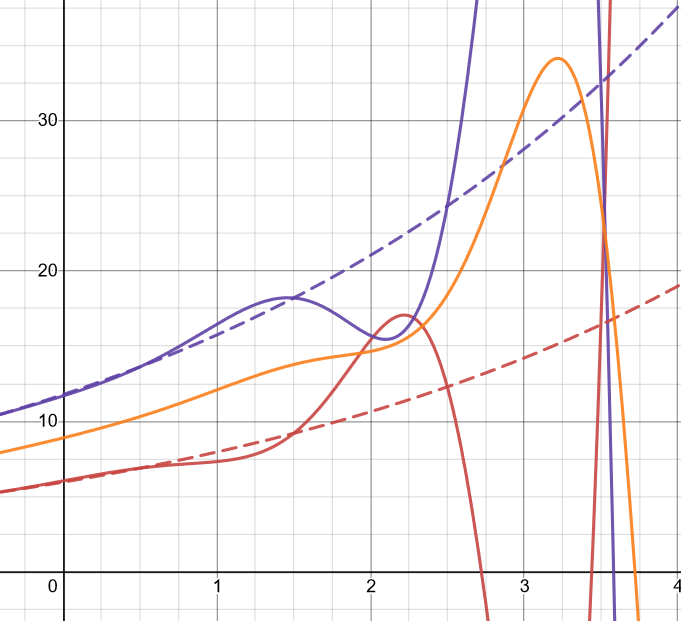
\includegraphics[scale=.7]{Images/netOutput}
\caption{The orange curve is the net output of society in terms of labor time.}
\end{figure}
 We can see in my figure here that the economy seems to expand beyond balanced growth bounds between periods $1$ and $2$, followed by a violent contraction. We can note with the orange curve $Y(t)$ that this does indeed correspond to an expansion and contraction in terms we would normally think of it. I don't have much else to say about this function right now but it will be helpful to look at occasionally as we go. \par 
The next three functions kind of go together.
\subsection{The Rate of Capital Accumulation}
 Let's start with $g_k(t)$, the rate of accumulation of capital. The function this represents is
\[ g_k(t) = \frac{(c_1+v_1)\Delta y_1(t) + (c_2+v_2)\Delta y_2(t)}{(c_1+v_1)y_1(t) + (c_2+v_2)y_2(t)} \]
where $\Delta y_i(t) = y_i(t+1)-y_i(t)$, i.e. it is the change in $y_i$ between periods $t$ and $t+1$. To make sense of this function, note that $(c_1+v_1)y_1(t)$ is the operating capital of department $1$, i.e. it is how much necessary time needs to go into this industry to keep it moving and generating surplus. Thus the numerator here gives us how much bigger or smaller the economy has gotten between periods $t$ and $t+1$, while the function as a whole puts this difference relative to the size of the economy originally. Thus if $g_k(t)=.5$, then the economy got $50$ percent bigger between periods $t$ and $t+1$, and so forth. (We are essentially thinking about capital accumulation in \emph{real terms}. Not as the accumulation of \emph{wealth}, but rather the accumulation of necessary social activity.) \par 
Since this is a percentage, it is going to appear much smaller and more muted compared to the functions we've looked at so far, which is why I recommended changing the scale of things earlier. The figure below give a good picture and the settings that produce it. (Disclaimer: These settings will produce something very similar but not exactly identical to the rest of the figures below.)
\begin{figure}[H]
\centering
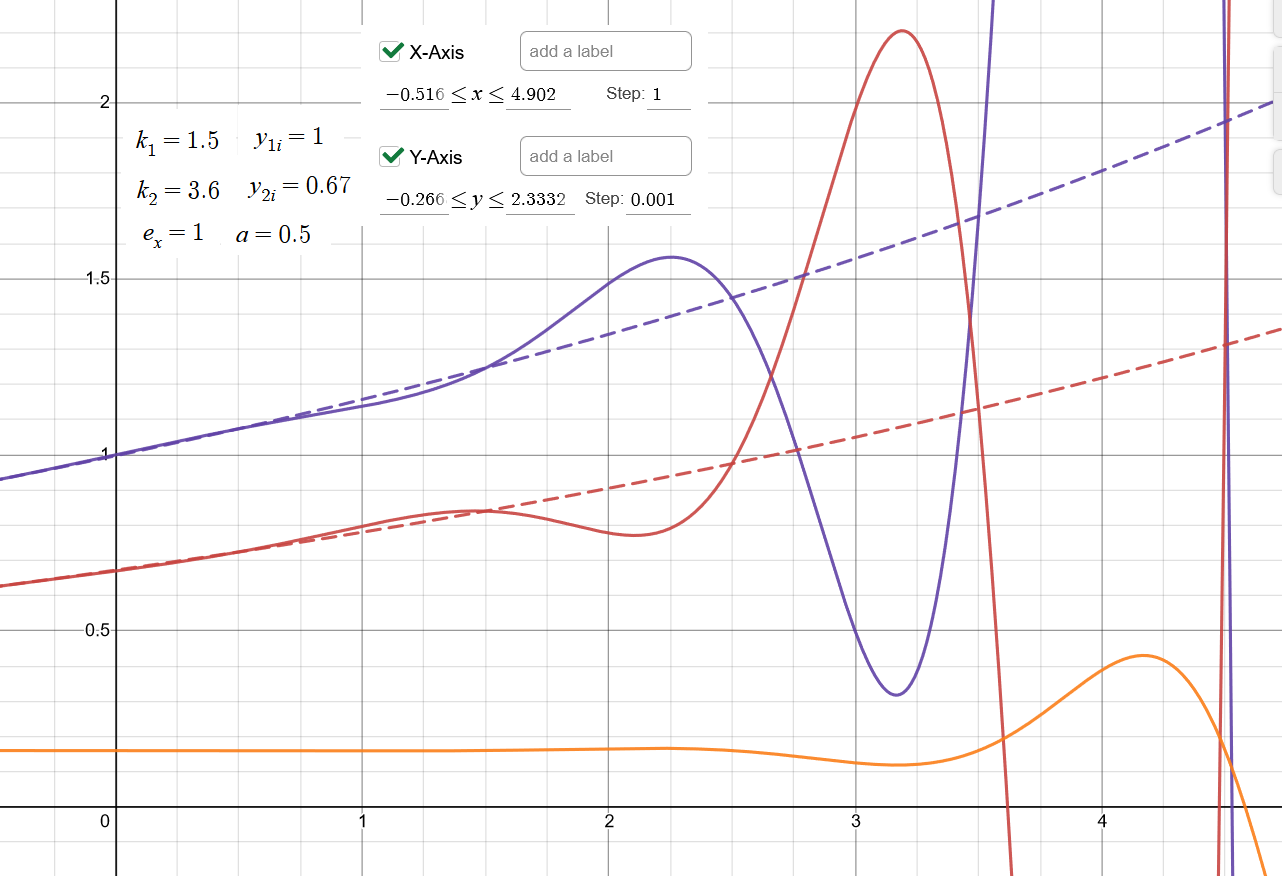
\includegraphics[scale=.6]{Images/rateOfAccumulation}
\end{figure}
To make sense of this, it's important to keep in mind that, the way we've defined it the rate of capital accumulation is continually forward facing, and it should be because it will play out based on how capitalists decide to invest at the \emph{beginning} of each production period. We can first see that between roughly period $1$ and period $2$, the economy convulses inward and then outward from the perspective of the almost balanced growth path. This is reflected in a small change in the rate of accumulation between periods $0$ and $1$. On my picture, this is too small to really see without clicking the curve and dragging the mouse along:
\begin{figure}[H]
\centering
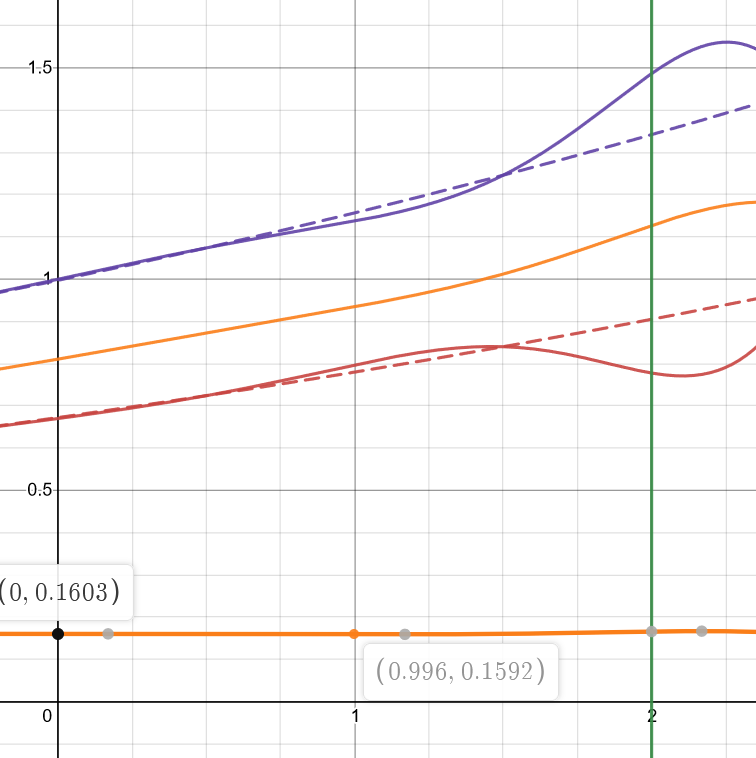
\includegraphics[scale=.7]{Images/dropInAccumulation}
\caption{Between periods 1 and 2, the more capital intensive industry declines, and this is mirrored in prior investment by a drop in the rate of capital accumulation between between periods $0$ and $1$, albeit by only about $0.1$ percent.}
\end{figure}
To make sense of this, we need to make an identification between the rate of accumulation and the rate of profit. Intuitively, this is a very simple relationship: I can only accumulate as fast as the rate at which I'm receiving profits to reinvest. If the rate of profit falls, then the rate of accumulation will also fall, provided that the rate of reinvestment remains the same. With our current settings, the wage goods department has a higher composition of capital and is thus more capital intensive than the capital goods department. This means that when society favors the wage goods industries, necessary costs rise, the amount of labor uses drops, and the profit produced per hour of labor also drops. Between periods 0 and 1, the wage goods department comes into favor. This is due to a shift in investment made at the beginning of period 0

we must keep in mind that the wage goods department has a higher composition of capital and is thus more capital intensive. We can see that by period 2, the capitalists have reinvested in such a way that the wage goods department has fallen out of paper. Thus prior to that, around period 1, we see a small slump in the rate of accumulation. On the other hand, we can see that the net output in labor time has slightly accelerated risen during this period, because, to repeat ourselves, labor intensive industries are on the rise. \par 
By period $3$ the situation has reversed. The more labor intensive industry collapses and the more capital intensive one soars. We thus see a rise in simultaneous dip in the net output in labor time $Y(t)$ and a rise in the rate of capital accumulation between periods $1$ and $2$. 
\begin{figure}[H]
\centering
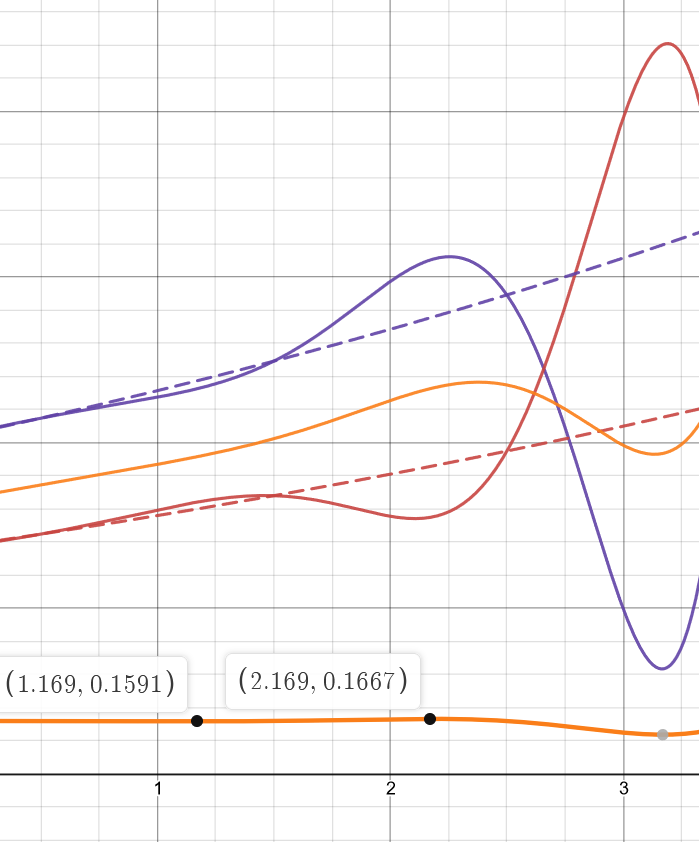
\includegraphics[scale=.7]{Images/slightRiseInAccumulation}
\caption{The labor intensive industries collapse and the capital intensive ones soar from periods $2$ and $3$, creating a dip in the net labor output $Y(t)$. This is all preceded in investment patterns between periods $1$ and $2$ corresponding to a rise in the rate of capital accumulation by about $.8$ percent.}
\end{figure}
These patterns repeat themselves, becoming more and more dramatic over time. Between periods $3$ and $4$ the labor intensive industries blast up again while the capital intensive ones collapse, and we observe in tandem with this a soaring of net output in labor time and a fall in the rate of accumulation between periods $2$ and $3$, this time by about $4$ percent. And so on. \par 
\subsection{Labor Demand}
Next, turn on the graphs of $D_L(t)$. This is the rate of change in the demand for labor:
\[ D_L(t) = \frac{l_1\Delta y_1(t)+l_2 \Delta y_2(t)}{l_1y_1(t) + l_2y_2(t)} \]
Recall that $l_i = v_i + s_i$. Thus $D_L(t)$ tracks the change in amount of labor needed in production from period to period. It's important to consciously acknowledge right away that if this is positive, even if unchanging, then more and more laborers are being brought into production each period. If it drops, but remains positive, then the workforce is still increasing in size, just at a lower rate. \emph{However}, if it at any point becomes \emph{negative}, then this would mean that workers are being laid off in significant numbers. Thus we should associate dips of this curve into the negative with mass layoffs. \par 
The first thing we should consider is the relationship between these two variables under stable circumstances. I've added in the next figure a few significant figures to the value of $y_{2i}$ to make things look closer to equilibrium. As we can see, in these conditions, Marx's famous adage holds true: accumulation of capital \emph{is} increase in the proletariat. $g_L(t) = D_L(t)$. 
\begin{figure}[H]
\centering
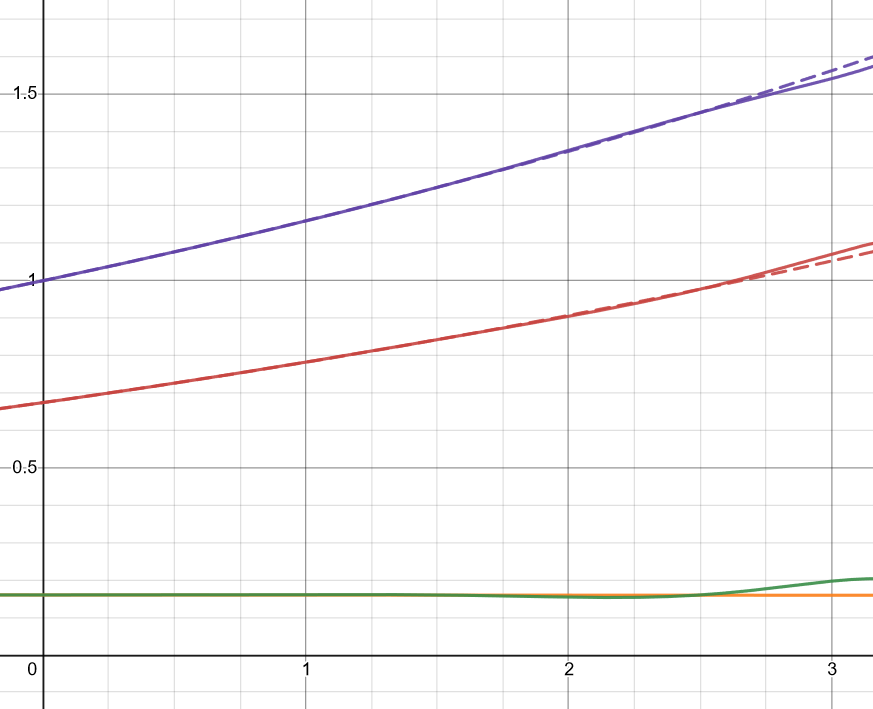
\includegraphics[scale=.7]{Images/accumulationOfProles}
\caption{In conditions of stable and balanced growth, the rate of accumulation and the rate of changing labor demand are identical.}
\end{figure}
However, when I take those significant figures away and go back to the old conditions, I see a picture that looks like this:
\begin{figure}[H]
\centering
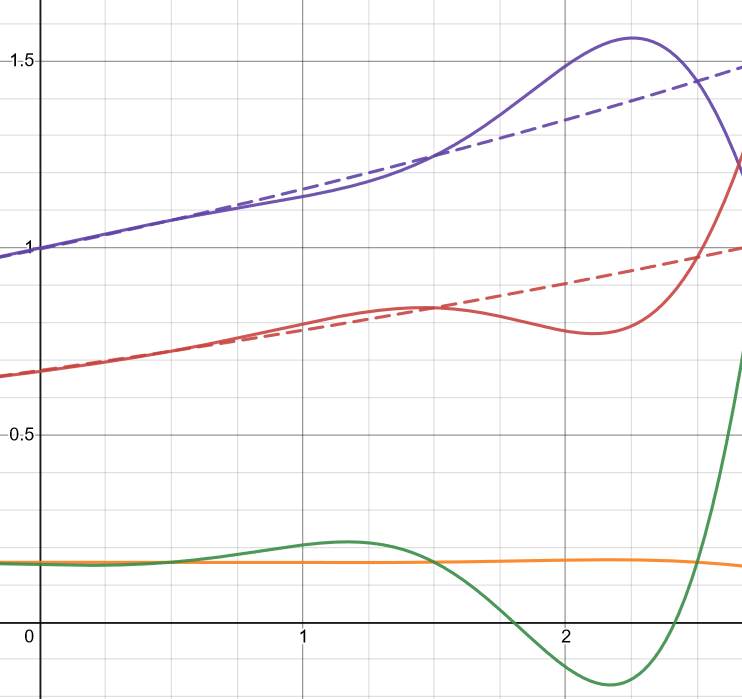
\includegraphics[scale=.7]{Images/accumulationDifferent}
\end{figure}
It would make sense that the demand for labor to change as the economy expands and contracts, but why is it changing separately from the rate of accumulation? Likewise, why was the net output in labor time doing the opposite of the rate of accumulation as industries fluctuated? The answer to both of these questions is: a changing \emph{overall} composition of capital.
\subsection{Composition of Total Social Capital}
 Now the composition of capital \emph{per department} doesn't change with the value output. The parameters $c_1$, $v_1$, $c_2$ and $v_2$ determine this because at any moment in time, the total constant capital in industry $1$ is $c_1y_1(t)$, and the total variable capital is $v_1y_1(t)$, and so
\[ \frac{c_1y_1(t)}{v_1y_1(t)} = \frac{c_1}{v_1} = k_1 \hspace{2cm} \frac{c_2y_2(t)}{v_2y_2(t)} = \frac{c_2}{v_2} = k_2 \]
Therefore on a \emph{per department} basis, the composition of capital can only change with changes in technology and labor productivity, which our model assumes is constant with time. However, the \emph{overall} composition of capital, i.e. the \emph{total} constant capital in society divided by the \emph{total} variable capital, is entirely different. This is the function $K(t)$ in Desmos, located underneath the rate of accumulation. 
\begin{figure}[H]
\centering
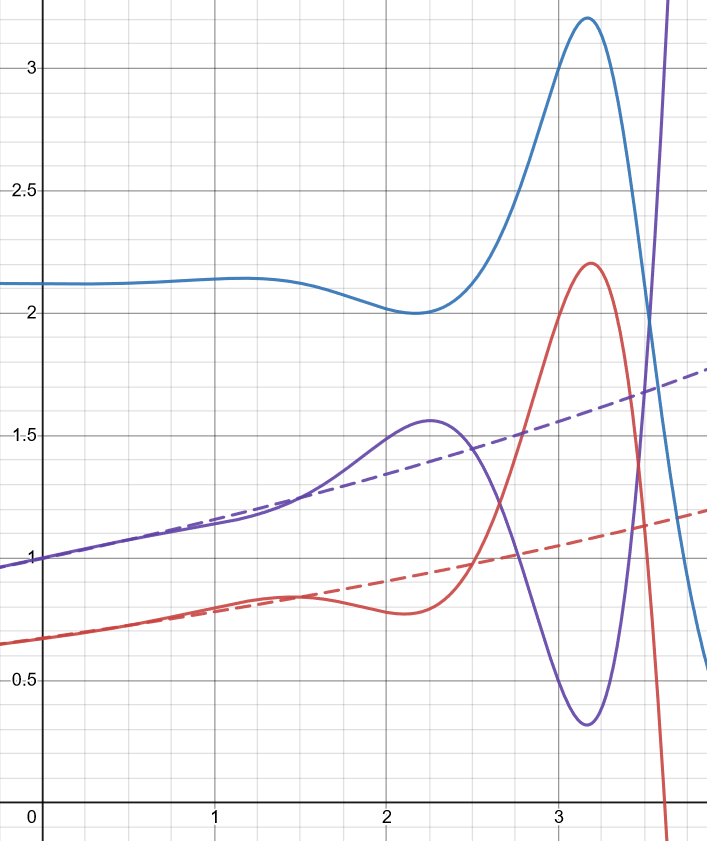
\includegraphics[scale=.7]{Images/composition}
\caption{The overall composition in capital is the blue curve.}
\end{figure}
The formula for the composition of capital is
\[ K(t) = \frac{c_1y_1(t) + c_2y_2(t)}{v_1y_1(t) + v_2y_2(t)} \]
Why would this change independently of technology? The reason is the difference between the compositions within the two departments. Consider the dip which it takes around $t=2$. This happens as the capital goods industry comes into favor, which of the two departments, has the lower composition of capital. Thus while technology has not changed at all, an inflated proportion of the economy is suddenly engaging in more labor intensive industries. The economy becomes skewed in favor of more. \par 
This dip naturally corresponds to an increase in labor demand, but this spike will be observable in the \emph{previous period} since the workers had to be hired earlier to create this inflated situation! This is extremely important but also a little bit cluttered so I've included figures both with and without the $y_i(t)$ curves displayed:
\begin{figure}[H]
\centering
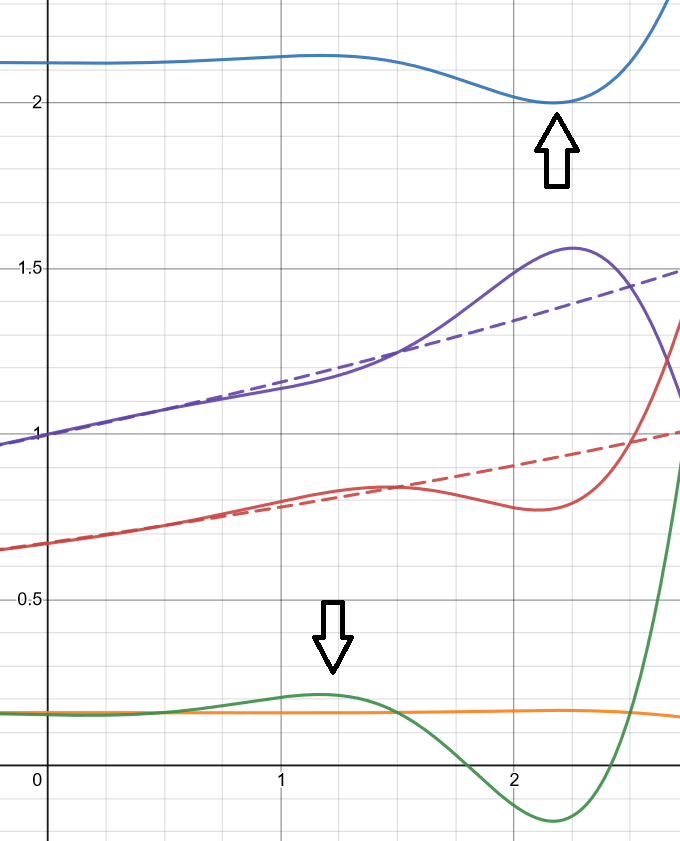
\includegraphics[scale=1]{Images/laborDemandWithCurves}
\caption{We see at $t=2$ an imbalance developing in which significantly more of societies time is being dedicated to the production of capital goods at the expense of the wage goods. The capital goods industry has a lower composition of capital, i.e. is the more labor intensive industry. Thus the consequence is a drop in the overall composition of capital, represented by the blue curve. Creating all of this is an investment boom for the capital goods industry - i.e. a period of time in which labor demand soars. This soaring of labor demand happens \emph{before} any of the changes mentioned, it is why this happens later!}
\end{figure}
But we know what happens next. The overproduction of capital goods and underproduction of wage goods creates an even more violent turn in the other direction. By the next period, society will be even more skewed, but this time in favor of the wage goods department, the more productive of the two. Demand for labor plummets, and this time manages goes negative. The industry swing is thus preceded with mass layoffs and skyrocketing unemployment.
\begin{figure}[H]
\centering
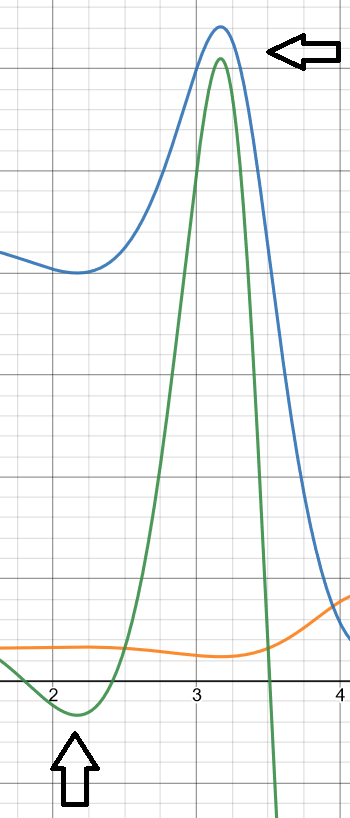
\includegraphics[scale=.7]{Images/demandSpike2}
\caption{The spike in composition a bit after $t=3$ is preceded with a plummeting of labor demand a bit after $t=2$, i.e. it is the \emph{result} of mass layoffs. The next swing is inevitably worse, and this means a bigger swing in labor demand then before.}
\end{figure}
A few things are noteworthy here. First, the explosive nature of these oscillations means that each swing in demand will be worse than the next. Thus it is \emph{guaranteed} that more workers will be laid off than were hired during the previous period in which labor demand spiked. You could say that it goes in the other direction as well - that the next spike in labor demand will involve more hiring than there were layoffs - but as we've noted repeatedly, it is likely this second big swing which triggers a crisis. At that point, things will be reset to some kind of equilibrium. At that point, labor demand will be made positive again, but it will be steady and unchanging - not a massive spike which immediately provides new work opportunities for the hungry workers. Moreover if the next round of economic earthquakes comes before all of these workers have been rehired, then we will arrive at Marx's theory of the increasing reserve army without any mention of technological change! We will soon bring in the factor of technological change, which can be seen to either substitute for the assumption of sufficiently bad initial conditions following crises or supplement the overall argument. \par 
\subsection{The Curious Case of $k_1 > k_2$}
 Before that however, we should remember not to get ahead of ourselves, because these solutions look vastly different if the composition of the capital for the capital goods department exceeds that of the wage goods department. In this case we have one great explosion of output in opposite directions. Within this situation we have two cases to consider: the case in which we begin with an oversupply of capital goods and an undersupply of wage goods, and the case in which we begin with an oversupply of wage goods and an undersupply of capital goods. Recall that in either case, capitalists have no choice but to double down and make the situation worse and worse for themselves. (See section 1 for the intuitive argument of why this rather counterintuitive scenario is bound to play out.)
\begin{figure}[H]
\centering
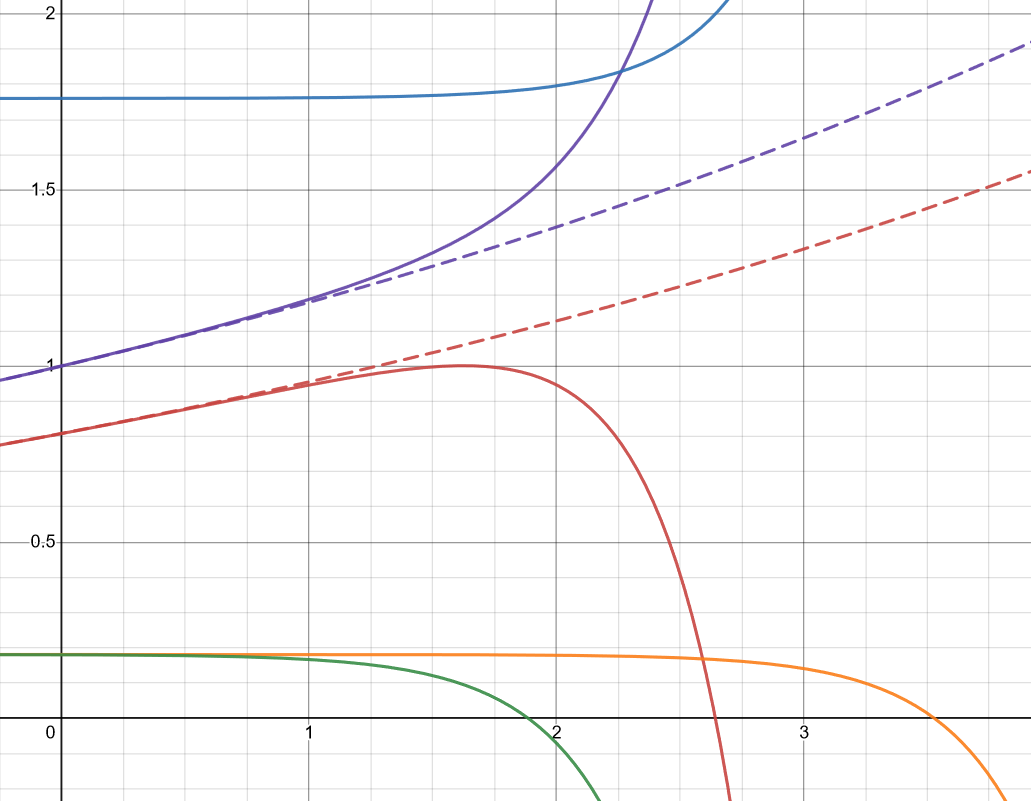
\includegraphics[scale=.7]{Images/divergenceEZCase}
\caption{Case 1: We begin with slight overproduction of capital goods.}
\end{figure}
Here we begin with a slight overproduction of capital goods at the expense of wage goods. Since the capital goods industry is assumed to have the higher composition of capital, we see the accompaniment of a ballooning overall composition of capital. Therefore labor demand goes into free fall, plummeting into the negative before the second period even begins. The mass layoffs simply continue until capitalists admit there is a crisis and reconfigure things. Case two is more interesting.
\begin{figure}[H]
\centering
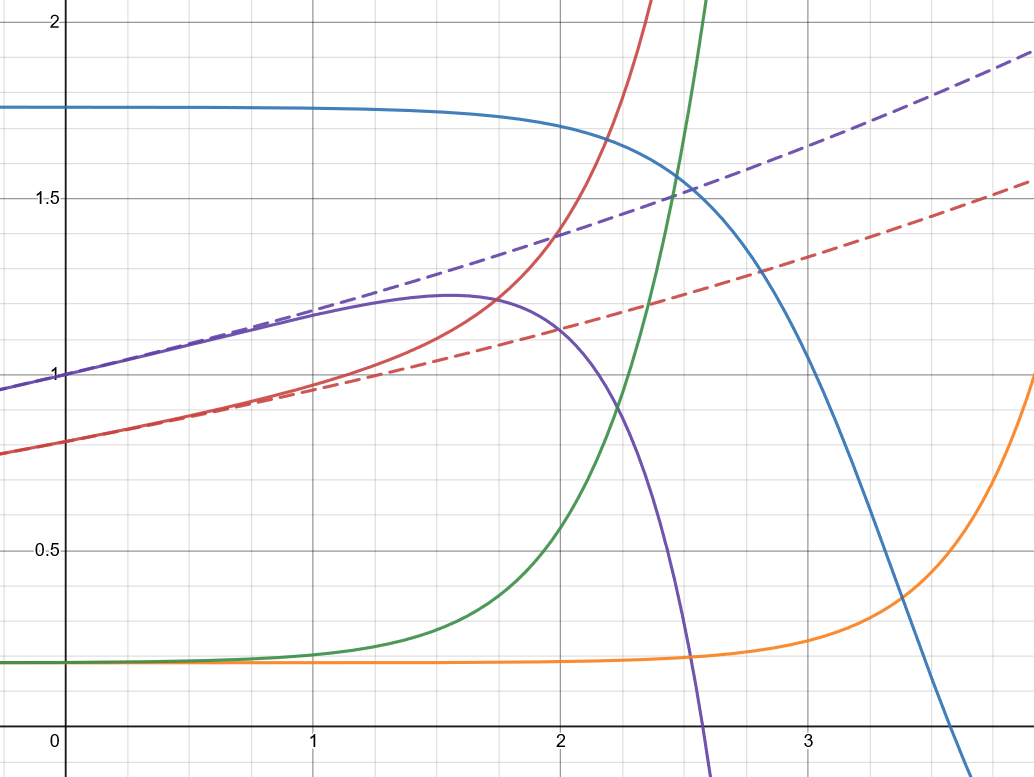
\includegraphics[scale=.7]{Images/divergenceHardCase}
\caption{Case 2: We begin with a slight overproduction of capital goods.}
\end{figure}
In case two we see continually exacerbating overproduction of wage goods at the expense of the capital goods. Since wage goods are the more labor intensive industries, this corresponds to a \emph{falling} composition of capital and therefore a perpetually \emph{rising} demand for labor. Thus we are facing a very peculiar crisis here, in which workers being laid off in the capital goods industry are immediately finding work in the wage goods industry, and beyond even this we see perpetually rising employment. Thus the nature of the crisis is going to be significantly different than the others. Let's consider the differences. \par 
Before, in the case of oscillations, we had capitalists going out of business and workers being laid off left and right. Things were so hectic that considering the fine details of \emph{why} the situation corresponded to a crisis didn't seem worth our time. Here things are very peculiar. First, there is no clear crisis of overproduction. We call the situation `overproduction of wage goods', but the continually expanding labor demand means more and more workers are being brought into the system and supplying effective demand for the products. Really it's less overproduction of wage goods and more an imbalance in which capital goods are continually perceived as more and more valuable. It's also not clear that any capitalists are going bankrupt. Capitalists engaged in wage goods will want to shift their capital to capital goods but won't be able to because doing so would involve increasing their composition of capital in a situation in which capital goods are in short supply. Thus the situation will present itself less as a stream of bankruptcies and more as a process in which a shrinking class of elite capital goods producers gradually creates for itself an increasing stake in the wage goods department and dominate the whole system. As they do this they'll start closing down their capital goods factories altogether as the cost of operation makes them unprofitable. Thus this crisis will manifest itself completely different from the other three. It will likely take the form of either a resource crisis (some kind of lashing out at neighboring countries for cheaper resources), or as a profit squeeze crisis, as the ballooning demand for labor gives workers more and more power. We haven't even discussed the effects of a rising or falling rate of exploitation on the situation. By moving the slider we can see that a rising value of $e_x$ could potentially reverse the situation, while the more likely scenario - a falling one, merely exacerbates the problems being discussed. \par 
These things are all, needless to say, incredibly interesting. It's truly striking how different this situation is from the other three. Because of this it seems to me extremely important that Marxists try to determine which department truly has the higher composition of capital. Moreover, one final observation about both these cases can potentially connect this task to the analysis of history. We noted that, when technology is such that capital goods are more capital intensive than wage goods, which of the two cases we get depends on the initial conditions $y_{1i}$ and $y_{2i}$. If the system is started off such that we have underproduction in wage goods and overproduction in capital goods, then we are locked into a situation in which capital goods are continually more and more favored. When the crisis hits, likely due to mass unemployment, we will be left with even more severe underproduction in wage goods and overproduction in capital goods. Thus the resetting process will likely involve the destruction of a large stock of capital goods. But if this only resets things somewhat and the situation is left with imbalance in the same direction as before, then the \emph{same} situation is what will repeat itself. Thus it seems at first glance like whichever of the two cases we get will be the case we continue to get, with no opportunity for switching to the other case from crisis to crisis. To analyze the situation further would be to analyze the way that states have reacted to crises in the past, so I'll leave it at that. The observation seems meaningful though that whichever case we have of these two seems like the natural candidate for the post-crisis situation.
\par 
\subsection{The Effects of Changing Technology}
Marx made none of these observations since he exclusively was interested in the balanced growth situation. His theory of the reserve army was thus entirely an argument based on changing technology. We can, to a somewhat limited extent, witness the effects of this within the Desmos app. It is extremely difficult to analyze the effects of changing technology outside of balanced growth, since the curves change so dramatically and drops in labor demand tend to move around as technology develops. Thus, let us first set things balanced by setting $y_{2i} = b_{g1}$ as before.
\begin{figure}[H]
\centering
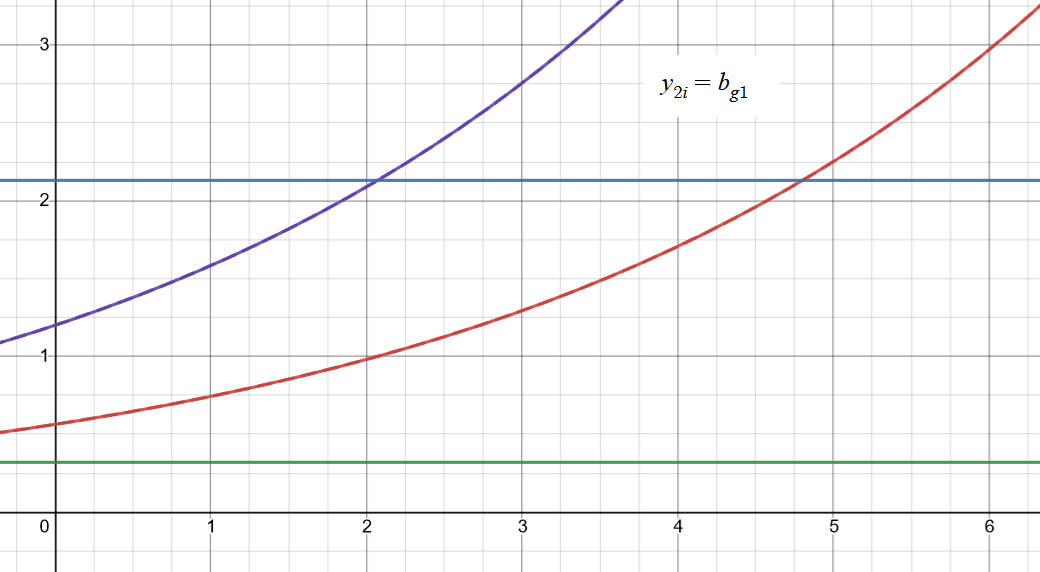
\includegraphics[scale=.7]{Images/backToBalanced}
\caption{Back to balanced growth we go. Note that along this path, the composition of capital, labor demand and the rate of accumulation are all constant, with $g_K(t) = D_L(t)$.}
\end{figure}
Here in the balanced growth situation, we can easily see the effects of an increasing composition of capital independent of crises in circulation. Simply zoom in on the $y$-axis enough to detect small changes in $D_L$, then move up either of the $k_i$ sliders to see the composition of capital and the demand for labor move away from one another. The former goes up, the latter goes down.
\begin{figure}[H]
\centering
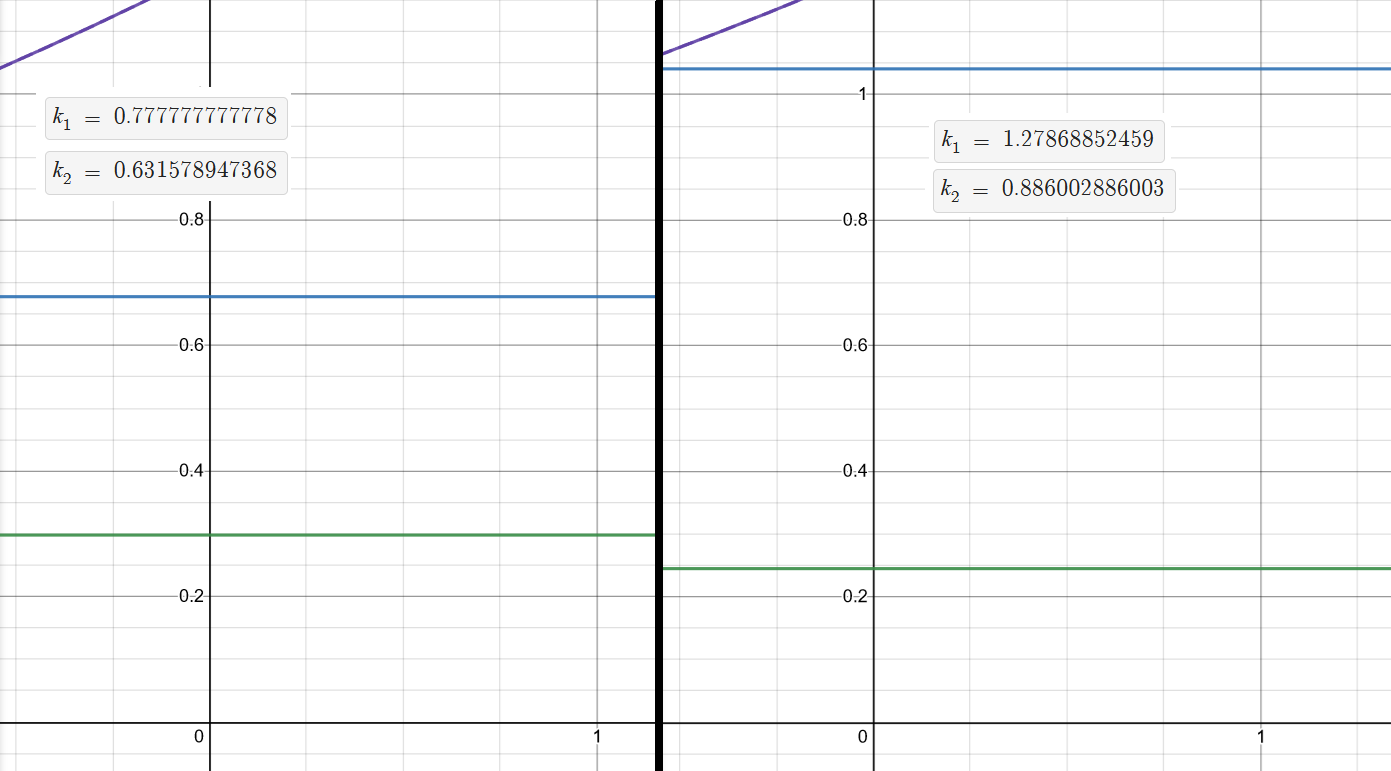
\includegraphics[scale=.5]{Images/fallingDemand}
\caption{It doesn't matter which composition you change. If either of the $k$ variables goes up, demand for labor goes down.}
\end{figure}
Thus, provided technological change under capitalism has the appropriate biases to cause an overall increase in the composition of capital of both departments, there will be an overall decline over time in the demand for labor. It follows that as workers are repeatedly laid off en masse as a result of the periodic crises we've been discussing, it is unlikely that the recovery will make up for the previous drop, and the result will be a growing reserve army. This results in a gradual decline in the bargaining power of labor over capital and subsequently a rising rate of exploitation, and this rising exploitation can only go so far before provoking open rebellion from the workers. That's how the story from volume 1 would go, anyway. \par 
Recall that the rate of accumulation is identical to labor demand if the composition of capital isn't changing, which as we can see is indeed the case when balanced growth is achieved. With that curve being identical to labor demand, it follows that a growing composition of capital also creates a gradually falling rate of accumulation. This can be seen as a foreshadowing of the falling rate of profit, Marx's other argument connected to the composition of capital. 
\subsection{Two useful equations}
Before turning to that though, let's provide some clarity to the observations we've been making with formulas. Firstly, it can be shown that for any $t$ we have
\begin{align} 
	1+D_L(t) = \frac{K(t)+1}{K(t+1)+1}(1+g_K(t)) \label{accumulationAndLabor}
\end{align}
It follows that as long as $K(t)$ is unchanging, we will have $D_L(t) = g_K(t)$. Accumulation of capital is increase in the proletariat. The more interesting formula comes next. It can also be shown that
\begin{align}
	 D_L(t) = \frac{ae-\Delta K(t)}{K(t+1)+1} \label{demandFormula}
\end{align}
where $\Delta K(t) = K(t+1)-K(t)$. The derivations of these equations can be found in appendix A. They require a bit of effort but don't involve anything fancy. Equation \ref{demandFormula} looks a little wonky but is extremely insightful. Both formulas tell a portion of the story about $D_L(t)$ and it's relationship with the composition of capital. Equation \ref{accumulationAndLabor} tells us that if the composition of capital isn't changing, there is no difference between $D_L$ and $g_K$, which is the first thing we observed visually. Equation \ref{demandFormula} tells us what happens if $K(t)$ \emph{is} changing. It tells us that an increase in $K$ creates a decrease in $D_L$, which we've also seen. What is new here is that it gives us precise conditions for when the demand goes negative. $D_L(t)$ becomes negative precisely when the increase in $K(t)$ exceeds the product of the rate of exploitation and the average rate of reinvestment. This means that the drop in labor demand can be offset by a rising rate of exploitation. It can also be offset by increasing investment, but the degree to which this can help is limited because investment can't go above $100$ percent. $e$ also has a maximum, presumably - namely when it gets so high that workers are collapsing and dying on the job, or more hopefully when they get fed up and revolt. 
\section{The Rate of Profit}
\subsection{The Transformation Problem}
Finally, we turn to the rate of profit. Or we should rather say, rates of profit, because there are $5$ of them, along with $2$ more function related to them. Go ahead and turn on the $P_1,P_2,P,P_b,P_g,T_b$ and $T_p$ functions. As long as you're in the $k_1 > k_2$ situation from the previous section they shouldn't look that bad when they're all on together. We'll discuss them one at a time. 
\begin{figure}[H]
\centering
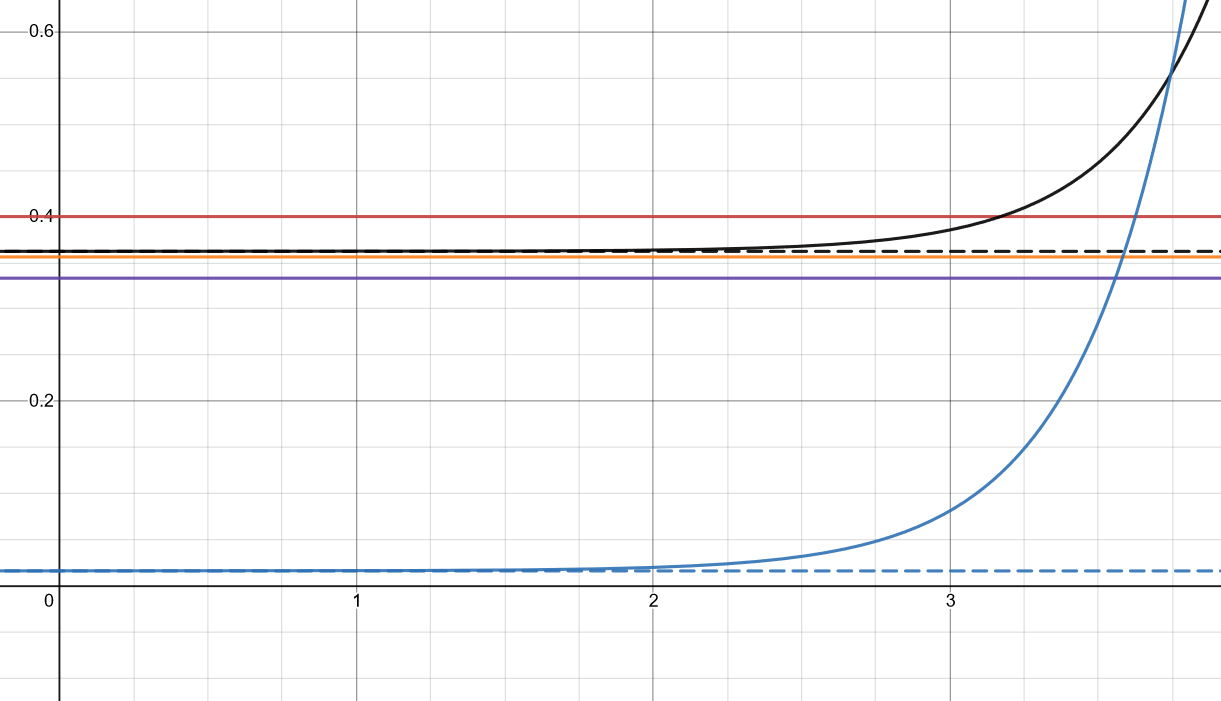
\includegraphics[scale=.5]{Images/ratesOfProfit}
\caption{There's a lot going on here.}
\end{figure} 
Before discussing any of these it is important to emphasize that we are assuming that an equilibrium \emph{money} rate of profit prevails in society, and that despite our discussions about it, the warranted paths operate as they do regardless of the reality of supply and demand, and assumes that the two are in constant equilibrium. The rates of profit graphed are \emph{not} money rates of profit, but rather \emph{value} rates of profit, since everything we are graphing is in value terms, not money terms. First, we have the purple and red lines, $P_1$ and $P_2$, which represent the rates of profit for the two departments. These are constant for the same reason that the per-department composition of capital was constant: 
\begin{align}
	& P_1(t) = \frac{s_1y_1(t)}{c_1y_1(t)+v_1y_1(t)} = \frac{s_1}{c_1+v_1} \\
	& P_2(t) = \frac{s_2y_2(t)}{c_2y_2(t)+v_2y_2(t)} = \frac{s_2}{c_2+v_2} 
\end{align} 
Next we have the black lines. The dotted black line is the rate of profit along the balanced growth path. It seems a bit difficult to show, but being on the balanced growth path means the value rate of profit is constant. The solid black line is the actual rate of profit along the actual growth path. It is given by the equation:
\begin{align}
	P(t) = \frac{s_1 y_1(t) + s_2y_2(t)}{(c_1+v_1)y_1(t) + (c_2+v_2)y_2(t)}
\end{align}
 Just as the actual growth path sticks to the balanced one before exploding away from it, the `real' value rate of profit sticks to the balanced growth path before blasting away with it as we would expect. \par 
However, \emph{neither} of these black lines are generally going to be the \emph{actual} money rate of profit that the capitalists experience. The \emph{money} rate of profit is also constant, but that is an assumption of the model. This is the famous problem with Marx's transformation from volume $3$. Marx claimed there that the total surplus value produced by society was redistributed among the capitalists in such a way that everyone received equal returns for equal investments (provided supply and demand were in equilibrium). If this were the case, then individual capitalist industries (and different departments) might have different value rates of profit, but would nonetheless experience the same money rates of profit, and would be oblivious to the former. However, since this is accomplished by a mere redistributing of the surplus value, it should be the case that the total value rate of profit of society as a whole (i.e. the thing we are tracking) is still equal to that money rate of profit that the capitalists experience. \par 
It can be shown that if the rate of profit has been equalized across all industries, then in a model like ours there is only a single positive number that the equilibrium \emph{money} rate of profit can be. Furthermore, that single number turns out to be the balanced growth path rate value of profit in the extremely special case where \emph{all surplus is reinvested}. That is to say, nothing is consumed by capitalists. This is the number $\pi_g$ in Desmos, and the function plotting that value alongside the other ones is $P_g$ (the orange line). We can see for ourselves that the balanced growth path rate of profit approaches this golden line as capitalist consumption approaches $0$ by moving the $a$ slider all the way to $1$. 
\begin{figure}[H]
\centering
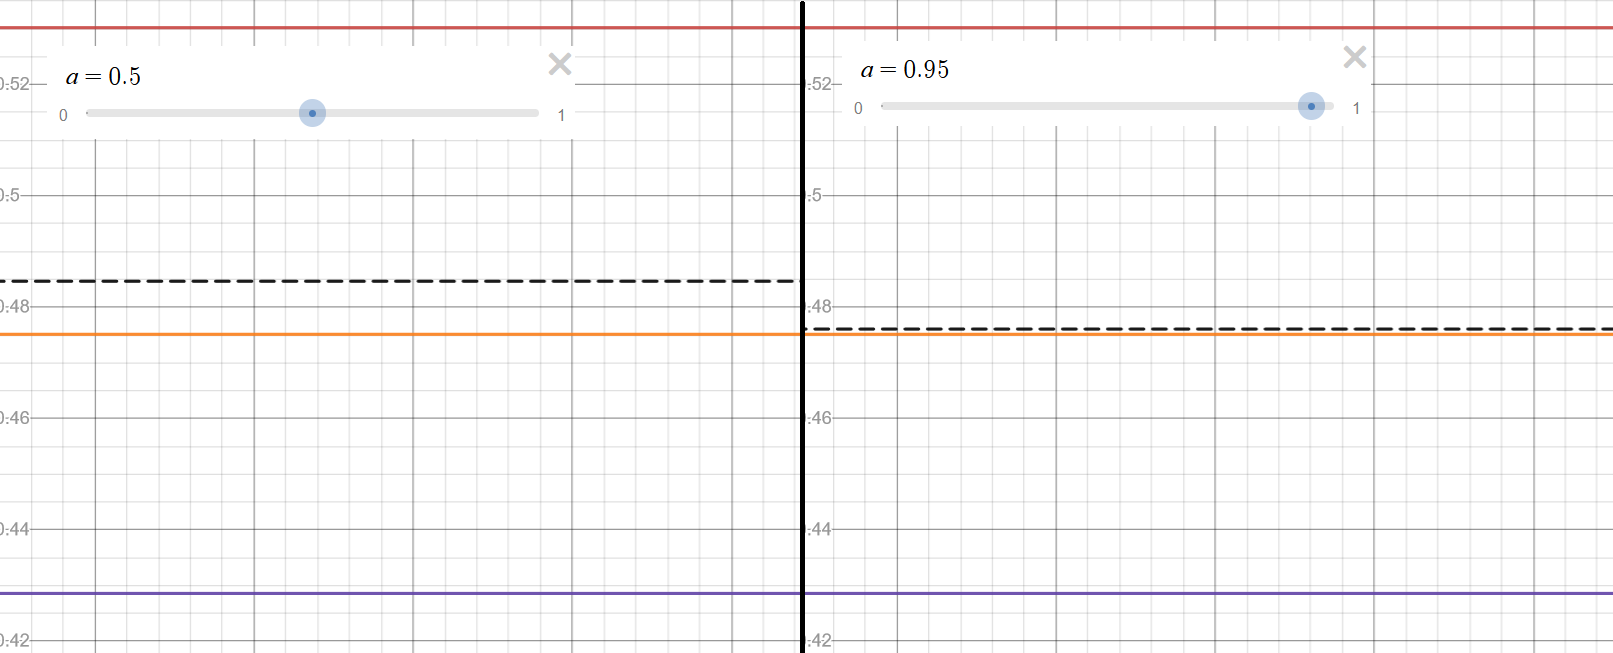
\includegraphics[scale=.5]{Images/approachingGolden}
\caption{As capitalist consumption approaches $0$, the total societal value rate of profit along the balanced growth path approaches the money equilibrium rate of profit.}
\end{figure}
Thus as long as capitalists consume some of their surplus, Marx's claim cannot be true in the strictest sense; the total surplus value divided by the total value of the constant and variable capital cannot equal the prevailing money rate of profit that capitalists are experiencing. This is true \emph{even if} capitalists are supposedly traveling along the balanced growth path. To leave it at this is to make it seem like Marx's argument is completely destroyed. However... \par 
First let's note that along the balanced growth path, even though the value rate of profit isn't generally \emph{equal} to the equilibrium rate of profit, it is usually \emph{extremely close}. Even in the reverse extreme case, where $a=0$, i.e. when capitalists consume \emph{all} of the surplus, the difference here in my model is only about $0.02$, a $3$ percent difference from the actual thing.
\begin{figure}[H]
\centering
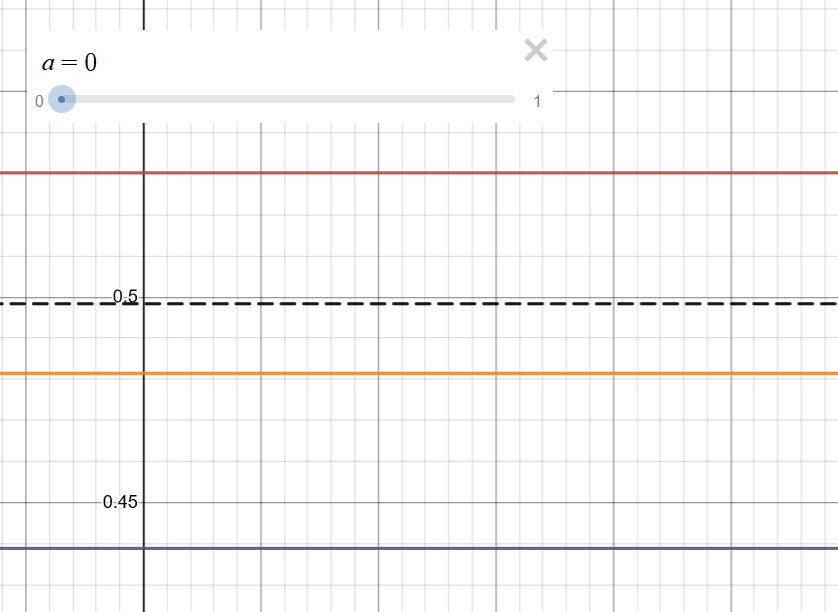
\includegraphics[scale=.7]{Images/reverseExtreme}
\caption{Even as capitalist consumption approaches $1$, the value rate of profit is along the balanced growth path is extremely close to the money rate of profit experienced by capitalists.}
\end{figure}
The function $T_b(t)$ measures this difference in relative terms (i.e. it gives the difference as a proportion of $\pi_g$). From what I can tell there are two major factors that make this difference get bigger, aside from a shrinking rate of reinvestment. One is exploitation. Sliding this up will have a modest effect separating these numbers. The other is the difference between the two departmental compositions of capital. Interestingly, this also determines whether $T_b$ is positive or negative. If $k_1 > k_2$, then $P_b$ is bigger than $\pi_g$, i.e. the value rate of profit overestimates the money rate. If $k_1 < k_2$, then $T_b$ dips negative, i.e. the value rate underestimates the money rate. Perhaps most interestingly, if $k_1=k_2$, then the two rates are equal, which is famously the condition that Samuelson identified, from which he concluded that everything Marx did was garbage. The idea that all industries have identical compositions of capital is of course ridiculous - Samuelson is correct about that - but he failed to identify this second condition we've identified: that it is also achieved along the balanced growth path when capitalists don't consume, \emph{regardless} of the compositions of capital. We will see why this is the much more important observation. Morishima also notes that the condition of $k_1=k_2$ can actually be relaxed somewhat to what he calls `linearly dependent industries', but I'm not sure how that condition translates to our aggregated departmental model. It might not functionally mean much.
\begin{figure}[H]
\centering
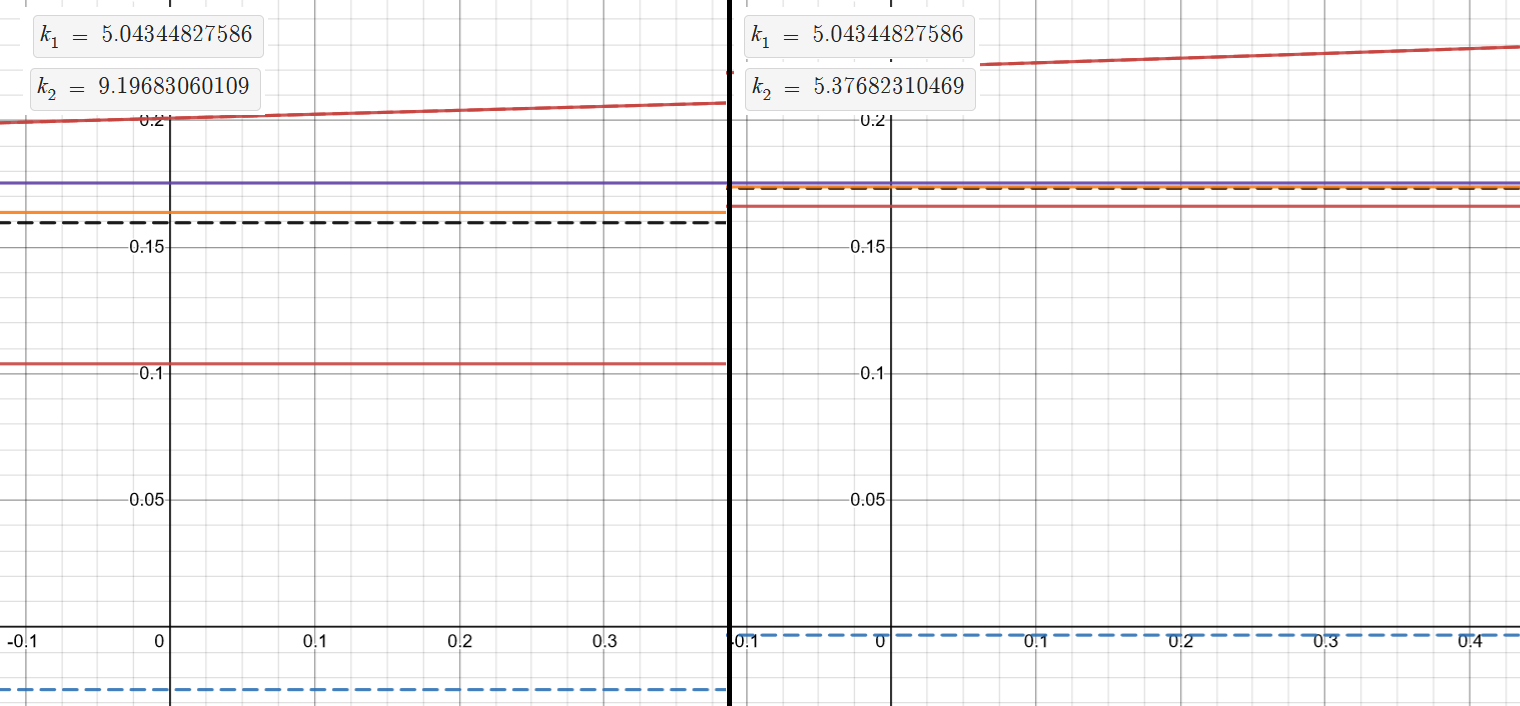
\includegraphics[scale=.5]{Images/relativeDiff1}
\caption{The broken blue line represents the relative difference between the value rate of profit along the balanced growth path and the equilibrium money rate of profit that capitalists experience. These are equal when $a=0$, but also approach equality as $k_1$ approaches $k_2$. We can see simultaneously all of the rates of profit become squashed together as this happens. When $k_2 > k_1$, the value rate underestimates the money rate, while when $k_2 < k_1$, it overestimates.}
\end{figure}
Why is this significant? Because we've been assuming that with every crisis, \emph{things get reset back to something approximating a balanced growth path}. And we just got done explaining why the balanced growth path has a value rate of profit that is usually very close to the actual equilibrium money rate of profit. Therefore we can conclude that \emph{outside times of crisis, Marx's claim from volume $3$ is generally very close to the truth}. That is to say, in times of relative calm the aggregate rate of profit for all of society is generally a very good approximation of the actual money rate of profit. The function $T_p$ tracks the relative difference. \par
\begin{figure}[H]
\centering
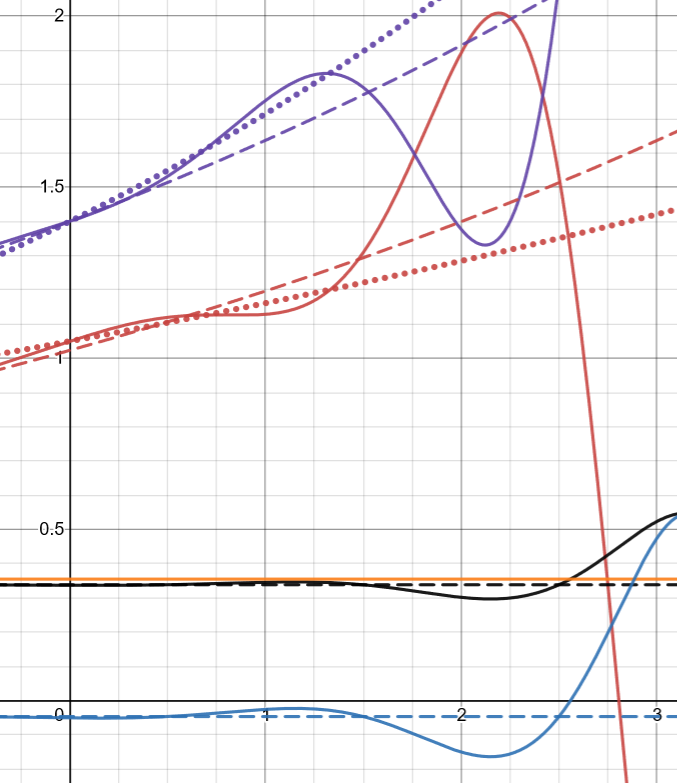
\includegraphics[scale=.8]{Images/theTransformation}
\end{figure}
In the figure above, we see the full story of a business cycle. The system is started off imperfectly, with just a bit of disparity from the balanced growth path. This disparity is small enough that the warranted path allows for mostly balanced growth in the first period, and this balanced growth itself lines up with what we started out with assuming that capitalists would naturally try to do with their surplus. We can see during this $0^{th}$ period of relative stability that the relative difference between the value rate of profit and the equilibrium money rate of profit is around very small. It is about a $5$ percent underestimate at the beginning of the period, and by the end of the period it actually falls to just $2$ percent (it improves!). By the end of period $0$, we begin to see capitalists favoring the capital goods industry at the expense of the wage goods industry in response to the availability of resources. Following this is the first real earthquake - a wild kneejerk shift in the opposite direction. At this point, that is by period $2$, the warranted path has diverged significantly from the balanced growth path, and this produces a significant different between the value rate of profit and the money rate of profit. However, even here, it's only $15$ percent off! To keep the economy on it's current trajectory would send things collapsing into total free fall, and therefore at this stage we would expect a state to step in and do whatever is necessary to restore something close to balanced growth. The process repeats. \par 
Thus over the course of this entire cycle of crisis, from boom to bust, the value rate of profit was at best $98$ percent representative of what capitalists were actually experiencing, and at worst still $85$ correct. There is certainly a lot of truth to Marx's argument! It's just not the full story. 
\subsection{The Technology Induced Falling Rate of Profit}
Lastly, we consider Marx's argument for the rate of profit to fall over time. This can be done rather easily, but only crudely. We can proceed identically to how we did when looking at labor demand: set the system off in perfect balanced growth conditions so that we can observe the effects of a changing composition independently of the unstable course of development. \par 
Everything you would expect to happen happens. It rises with a rising rate of reinvestment as well as a rising rate of exploitation, and, just as we'd expect, it falls as the composition of capital for either industry rises. This happens whether we are talking about the value rate of profit or the money rate of profit. Despite them not being the same, both do indeed fall at the same rate as the composition increases. 
\begin{figure}[H]
\centering
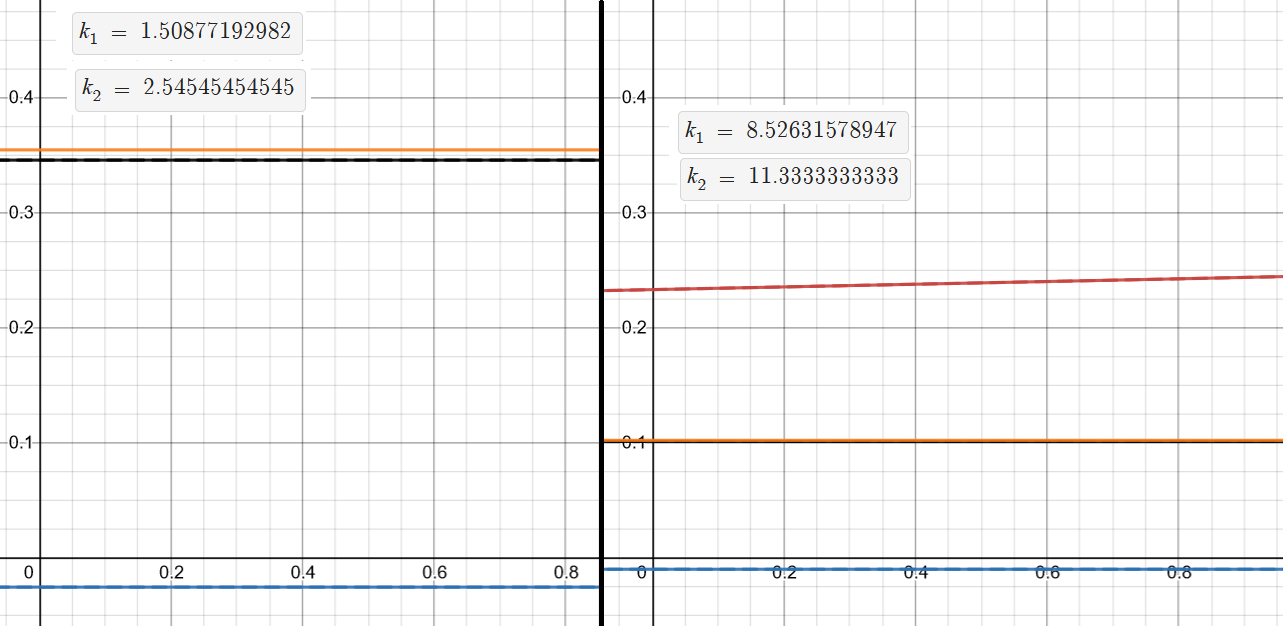
\includegraphics[scale=.6]{Images/theFallingRatesOfProfit}
\caption{As the compositions of either department increase, the overall composition increases and with it the rate of profit falls, whichever rate you might be considering. Note also that the relative difference between the value rate of profit and money rate of profit varies independently. You can make it as big as you want or as small as you want while simultaneously making the rate of profit itself as small as you want.}
\end{figure}
This is a very crude demonstration of the falling rate of profit because it assumes from the outset that the composition of capital is increasing. The real controversy surrounds what kinds of real technological changes \emph{actually} correspond to a falling rising composition. \par  
\section{Conclusions and Takeaways}
	Marx's presentation of his reproduction schema was an attempt to demonstrate the unlikeliness of capitalism's ability to engage in expanded reproduction in a stable way. He did a good job of this, an exceptional job for the time, but in his focus on this goal and his limited mathematical toolkit, he stopped just short of turning that argument into a model in which most of his other arguments can be framed and observed. What we get after doing this are a few cool takeaways. First, we get that the theory of the expanding reserve army can be framed independently of any argument about the compositions of capital changing. The mere sloshing around of the composition back and forth as a result of capitalists reconciling their desires for expanded surplus and available material resources will usually provide this on it's own. This is of course contingent on not being in that final case of the model we considered, in which $k_1 > k_2$ and the system is started off with an undersupply of capital goods. However this case itself is extremely interesting and produces crises of a completely different sort, but which are nonetheless very familiar to the history of capitalism. \par 
	Second, we get that Marx's transformation really isn't as wrong as it seemed at first. It's generally a surprisingly close approximation of the genuine article. Overall, it seems like everything pointed to by this dynamic model aids the overall argument Marx is making. While this isn't exactly \emph{his} reproduction schema, I believe it is a straight improvement and I would say the natural completion of what he sought out to do with it. I hope people found this little tour useful to their understanding of this stuff. It certainly helped me. I'm planning on continuing to expand the app in various ways. In particular I hope soon to create an alternative version of it in which capitalists are reinvesting in price terms rather than value terms. However, the dynamics in that situation should be mostly the same.
\subsection{Appendix A: Deriving the equations relating $g_K(t),D_L(t)$ and $K(t)$}\label{appendixA}
For all of what follows I'm going to ditch the functions of $t$ stuff. I'll fix a $t$ and let $g_K = g_K(t)$, $g_K' = g_K(t+1)$, and so forth. So we have 
\begin{align}
	& g_K = \frac{(c_1+v_1)\Delta y_1 +(c_2+v_2)\Delta y_2}{(c_1+v_1)\Delta y_1 + (c_2+v_2)\Delta y_2} \\
	& D_L = \frac{l_1\Delta y_1 + l_2 \Delta y_2}{l_1y_1 + l_2y_2} \\
	& K = \frac{c_1 y_1 + c_2 y_2}{v_1 y_1 + v_2 y_2} \\
	& P = \frac{s_1 y_1 + s_2 y_2}{(c_1 + v_1)y_1 + (c_2 + v_2) y_2}
\end{align} 
where $\Delta y_1 = y_1'-y_1$ and so forth. Note that
\begin{align}
	g_K &= \frac{(c_1+v_1)y_1' +(c_2+v_2)y_2' - [(c_1+v_1)y_1 + (c_2+v_2)y_2]}{(c_1+v_1)y_1 + (c_2+v_2)y_2} \\
	&= \frac{(c_1+v_1)y_1' +(c_2+v_2)y_2'}{(c_1+v_1) y_1 + (c_2+v_2) y_2} - \cancelto{1}{\frac{(c_1+v_1) y_1 + (c_2+v_2) y_2}{(c_1+v_1)y_1 + (c_2+v_2)y_2}} \\
	&=\frac{(c_1+v_1)y_1' +(c_2+v_2)y_2'}{(c_1+v_1) y_1 + (c_2+v_2) y_2} -1
\end{align}
Next note that 
\begin{align}
	K+1 = \frac{c_1 y_1 + c_2 y_2}{v_1 y_1 + v_2 y_2} + \frac{v_1 y_1 + v_2 y_2}{v_1 y_1 + v_2 y_2} = \frac{(c_1 + v_1) y_1 + (c_2 + v_2)y_2}{v_1 y_1 + v_2 y_2}
\end{align}
So that
\begin{align}
	P = \frac{s_1 y_1 + s_2 y_2}{(c_1 + v_1)y_1 + (c_2 + v_2) y_2} = e \frac{v_1 y_1 + v_2 y_2}{(c_1 + v_1) y_1 + (c_2 + v_2)y_2} = \frac{e}{K+1}
\end{align}
Noting that $l_i = v_i + s_i = (1+e)v_i$ we have
\begin{align}
	D_L &= \frac{(1+e)v_1\Delta y_1 + (1+e)v_2 \Delta y_2}{(1+e)v_1 y_1 + (1+e)v_2 y_2} \\ 
	&= \cancelto{1}{\left( \frac{1+e}{1+e} \right)} \frac{v_1 y_1' +v_2 y_2' - [v_1 y_1' + v_2 y_2']}{v_1 y_1 + v_2 y_2} \\
	&= \frac{v_1 y_1' +v_2 y_2'}{v_1 y_1 + v_2 y_2} - 1
\end{align}
Now if we add the one over and multiply by $1$ in the stupidest way imaginable, then rearrange:
\begin{align}
	D_L+1 &= \frac{v_1 y_1' +v_2 y_2'}{v_1 y_1 + v_2 y_2} \frac{\frac{(c_1 + v_1)y_1' + (c_2 + v_2)y_2'}{(c_1 + v_1)y_1' + (c_2 + v_2)y_2'}}{\frac{(c_1 + v_1)y_1 + (c_2 + v_2)y_2}{(c_1 + v_1)y_1 + (c_2 + v_2)y_2}} \\
	&= \left( \frac{v_1 y_1' +v_2 y_2'}{(c_1 + v_1)y_1' + (c_2 + v_2)y_2'} \right) \left( \frac{(c_1 + v_1)y_1 + (c_2 + v_2)y_2}{v_1 y_1 + v_2 y_2} \right) \left( \frac{(c_1 + v_1)y_1' + (c_2 + v_2)y_2'}{(c_1 + v_1)y_1 + (c_2 + v_2)y_2} \right) \\
	&= \left( \frac{1}{K'+1} \right) \left( K+1 \right) \left( g_k+1 \right) \\
	&= \frac{K+1}{K'+1}(g_K+1)
\end{align}
Therefore if $K = K'$ we have 
\begin{align}
	& D_L+1 = \cancelto{1}{\frac{K'+1}{K+1}}(g_K+1) \\
	&\implies D_L+\cancel{1} = g_K+\cancel{1} \\
	&\implies D_L = g_K 
\end{align}
confirming equation \ref{accumulationAndLabor}. For equation \ref{demandFormula}, we also know from the situation that all change in the accumulated capital must come from the re-invested surplus value from the prior period. I.e.
\begin{align} \label{surplusEquation}
	(c_1 + v_1) \Delta y_1 + (c_2 + v_2) \Delta y_2 = a(s_1 y_1 + s_2 y_2)
\end{align}
This isn't exactly obvious mathematically from how I `derived' my system for the warranted growth paths, but it can be shown and makes intuitive sense. Nonetheless it can be shown easily: First, since $y_1' = y_1 + \Delta y_1$ and $y_2' = y_2 + \Delta y_2$, we can re-express the system as 
\begin{align}
	& y_1 = c_1 y_1 + c_1 \Delta y_1 + c_2 y_2 + c_2 \Delta y_2 \\
	& y_2 = v_1 y_1 + v_1 \Delta y_1 + v_2 y_2 + v_2 \Delta y_2 + bs_1 y_1 + b s_2y_2
\end{align}
Next, by adding the two equations \ref{sys1} and \ref{sys2} and using the identity $c_i + v_i + s_i = 1$:
\begin{align}
	& y_1 + y_2 = c_1 y_1 + c_2 y_2 + v_1 y_1 + v_2 y_2 + c_1 \Delta y_1 + c_2 \Delta y_2 + v_1 \Delta y_1 + v_2 \Delta y_2 +bs_1y_1 + bs_2y_2 \\
	&\implies \cancelto{s_1}{(1-c_1-v_1)} y_1 + \cancelto{s_2}{(1-c_2-v_2)}y_2= (c_1+v_1) \Delta y_1 + (c_2+v_2) \Delta y_2 + b(s_1y_1 + s_2y_2) \\
	&\implies s_1 y_1 + s_2y_2 = (c_1+v_1) \Delta y_1 + (c_2+v_2) \Delta y_2 + (1-a)(s_1y_1 + s_2y_2) \\
	&\implies (a+b)(s_1 y_1 + s_2 y_2) - b(s_1y_1 + s_2y_2)=(c_1+v_1) \Delta y_1 + (c_2+v_2) \Delta y_2  \\
	&\implies a(s_1y_1 + s_2y_2) = (c_1+v_1) \Delta y_1 + (c_2+v_2) \Delta y_2 
\end{align}
Using this we can also rewrite $g_K(t)$ in a third way by replacing the numerator and using the fact that $s_i = e v_i$:
\begin{align}
	g_K &= \frac{a(s_1 y_1 + s_2 y_2)}{(c_1 + v_1)y_1 + (c_2 + v_2)y_2} \\
	&= ae \frac{v_1 y_1 + v_2 y_2}{(c_1 + v_1) y_1 + (c_2 + v_2)y_2} \\
	&= a\frac{e}{K+1} = a P
\end{align} 
Plugging this in to the equation from earlier for $D_L+1$ gives
\begin{align}
	D_L+1 = \frac{K+1}{K'+1}(g_K+1) &= \frac{K+1}{K'+1}\left( \frac{ae}{K+1} + 1 \right)\\
	 &= \frac{\cancel{K+1}}{K'+1}\left( \frac{ae + K +1}{\cancel{K+1}} \right) \\
	 &= \frac{ae+K+1}{K'+1}
\end{align}
Therefore 
\begin{align}
	D_L = \frac{ae+K+1}{K'+1} - \frac{K'+1}{K'+1} = \frac{ae+K-K'}{K'+1} = \frac{ae-\Delta K}{K'+1}
\end{align}
Which is exactly equation \ref{demandFormula}.
\subsection{Appendix B: Solving the system}
	To solve the system 
\begin{align}
	& y_1(t) = c_1y_1(t+1) + c_2y_2(t+1) \label{sys1} \\
	& y_2(t) = v_1y_1(t+1) + v_2y_2(t+1) + bs_1y_1(t) + bs_2y_2(t) \label{sys2}
\end{align}
will require some familiarity with linear algebra. In particular, we need to diagonalize a matrix. Firstly, we can rewrite this system as a matrix equation:
\begin{align}
	\begin{pmatrix} y_1(t) \\ y_2(t) \end{pmatrix} &= \begin{pmatrix} c_1 & c_2 \\ v_1 & v_2 \end{pmatrix} \begin{pmatrix} y_1(t+1) \\ y_2(t+1) \end{pmatrix} + \begin{pmatrix} 0 & 0 \\ bs_1 & bs_2 \end{pmatrix} \begin{pmatrix} y_1(t) \\ y_2(t) \end{pmatrix} \\
	&= \begin{pmatrix} c_1 & c_2 \\ \frac{bs_1c_1 + v_1}{1-bs_2} & \frac{bs_1c_2 + v_2}{1-bs_2} \end{pmatrix}\begin{pmatrix} y_1(t+1) \\ y_2(t+1) \end{pmatrix} \\
	&:= \begin{pmatrix} M_{11} & M_{12} \\ M_{21} & M_{22} \end{pmatrix}\begin{pmatrix} y_1(t+1) \\ y_2(t+1) \end{pmatrix}
\end{align}
To diagonalize the matrix $M$ is to find a basis on which $M$ acts `nicely'. If we find that, then we can re-express the system of equations in that new basis, solve it there, and then shift back into the standard one. This is the eigenbasis of the matrix, provided it has one. Assuming it does for the moment let $\mu_1$ and $\mu_2$ denote the eigenvalues of $M$ (in desmos they are $\theta_1$ and $\theta_2$). Through setting the determinant of $M-\mu I$ equal to 0, then applying the quadratic formula and simplifying the contents of the radical, we get
\begin{align}
	& \mu_1 =  \frac{1}{2}(M_{11}+M_{22}+\sqrt{(M_{11}-M_{22})^2 + 4M_{12}M_{21}}) \\
 & \mu_2 =  \frac{1}{2}(M_{11}+M_{22}-\sqrt{(M_{11}-M_{22})^2 + 4M_{12}M_{21}}) 
\end{align} 
Since all of the $M_{ij}$s are positive we can see immediately that $\mu_1$ is always positive. Furthermore since the radical is always positive, $\mu_1$ is more than halfway between the smaller and the bigger of $M_{11}$ and $M_{22}$, so it must be bigger than at least one of these. Note that there exists some $u>0$ such that 
\begin{align}
	\sqrt{(M_{11}-M_{22})^2 + 4M_{12}M_{21}} = |M_{11} - M_{22}| + u 
\end{align} 
since this is the distance plus some extra positive stuff inside the radical. Considering $\mu_2$ with this in mind, we see that we are taking the halfway point between $M_{11}$ and $M_{22}$, and subtracting away more than half the distance between them. Therefore $\mu_2$ may or may not be negative, but is always smaller than  both of $M_{11}$ and $M_{22}$. From the same argument we can also see that $\mu_1$ is \emph{bigger} than $M_{11}$ and $M_{22}$. When $\mu_1$ and $\mu_2$ are both positive, it is of course the case that $\mu_1 > \mu_2$. Suppose that $\mu_2$ is negative and that $\mu_1 < -\mu_2$. Then 
\[ \frac{1}{2}(M_{11}+M_{22}+|M_{11} - M_{22}| + u < -\frac{1}{2}(M_{11}+M_{22}-|M_{11} - M_{22}| - u \]
But this would imply that $M_{11} + M_{22} < 0$, which is a contradiction since all of these entries are positive. Thus we have the following facts known about the eigenvalues:
\begin{itemize}
	\item[(1)] $\mu_1 > 0$.
	\item[(2)] $\mu_1$ is bigger than both $M_{11}$ and $M_{22}$
	\item[(3)] $\mu_2$ is smaller than both $M_{11}$ and $M_{22}$
	\item[(4)] $\mu_1 > |\mu_2|$.
\end{itemize}
Next let
\begin{align}
	\vec{m}_1 = \begin{pmatrix} m^1_1 \\ m^1_2 \end{pmatrix}  \hspace{2cm} \begin{pmatrix} m^2_1 \\ m^2_2 \end{pmatrix}
\end{align}
denote eigenvectors associated with $\mu_1$ and $\mu_2$. These must satisfy the equations. (In desmos these are $m_{11}, m_{12},m_{21},m_{22}$.) 
\begin{align}
	& (M_{11} - \mu_1)m^1_1 + M_{12}m^1_2 = 0  \label{e11}\\
	& M_{21}m^1_1 + (M_{22} - \mu_1)m^1_2 = 0 \label{e12}
\end{align}
\begin{align}
	& (M_{11} - \mu_2)m^2_1 + M_{12}m^2_2 = 0  \label{e21}\\
	& M_{21}m^2_1 + (M_{22} - \mu_2)m^2_2 = 0 \label{e22}
\end{align}
We can see here that $M_{11} - \mu_1$ is always negative by observation $(2)$ earlier pertaining to the $\mu$'s, and so subtracting this term over and dividing we see that $m^1_1 = xm^2_1$ for some positive ratio $x$. Thus we can take the vector $\vec{m}_1$ as consisting of two positive entries. Namely let $m^1_1 = 1$, so that 
\begin{align}
	m_2^1 = \frac{\mu_1-M_{11}}{M_{12}}m^1_1
\end{align}
 Since $M_{11} - \mu_2$ is always positive, subtracting the term over and dividing gives that $m^2_1 = -xm^2_2$ for some positive $x$, and therefore we can take $\vec{m}_2$ as having a positive first entry and a negative second entry. In particular, again taking $m^2_1 = 1$, we have
 \begin{align}
 	m^2_2 = \frac{\mu_2-M_{11}}{M_{12}}m^2_1
 \end{align}
  Thus $\vec{m}_1$ points somewhere in quadrant $1$ and $\vec{m}_2$ points somewhere in quadrant $2$, which is enough to be sure they are linearly independent. It follows that $M$ has an eigenbasis, and thus is always diagonalizable, as long as both $\mu$ values are positive, which itself can be easily verified as the case as long as $k_1 \neq k_2$ (which is why my system breaks when you set them equal). Let 
\begin{align}
	 P = \begin{pmatrix} m^1_1 & m^2_1 \\ m^1_2 & m^2_2 \end{pmatrix} \implies P^{-1} = \frac{1}{m^1_1m^2_2-m^2_1m^1_2} \begin{pmatrix} m^2_2 & -m^2_1 \\ -m^1_2 & m^1_1 \end{pmatrix} 
\end{align}
Here seeing $P$ and $P^{-1}$ as change of basis matrices, $P$ takes vectors in the eigenbasis back to the standard basis, while $P^{-1}$ takes vectors from the standard basis into the eigenbasis. Let $\vec{y}(t)$ denote the pair of $y$ values in the standard basis, $\vec{z}(t)$ the vector in the eigenbasis, i.e. 
\begin{align}
	\vec{z}(t) = P^{-1}\vec{y}
\end{align}
Then $M = PDP^{-1}$, where 
\begin{align}
D = \begin{pmatrix} \mu_1 & 0 \\ 0 & \mu_2 \end{pmatrix}
\end{align} 
so that
\begin{align}
	& \vec{y}(t) = PDP^{-1}\vec{y}(t+1) = PD\vec{y}_{\mathcal{M}}(t+1) \\
	&\implies \vec{z}(t) = D\vec{z}(t+1) \\
	&\implies \begin{pmatrix} z_1(t) \\ z_2(t) \end{pmatrix} = \begin{pmatrix} \mu_1z_1(t+1) \\ \mu_1z_2(t+1) \end{pmatrix}
\end{align}
Letting $\eta_1 = z_1(0)$ and $\eta_2 = z_2(0)$ represent the initial values of $z_1$ and $z_2$ (in desmos they are $r_1$ and $r_2$), i.e.
\begin{align}
	 \begin{pmatrix} \eta_1 \\ \eta_2 \end{pmatrix} = \frac{1}{m^1_1m^2_2-m^2_1m^1_2} \begin{pmatrix} m^2_2 & -m^2_1 \\ -m^1_2 & m^1_1 \end{pmatrix} \begin{pmatrix} y_1(0) \\ y_2(0) \end{pmatrix}
\end{align}
Thus
\begin{align}
	& \eta_1 = \frac{m^2_2y_1(0)-m^2_1y_2(0)}{m^1_1m^2_2-m^2_1m^1_2} = \frac{(\mu_2-c_1)y_1(0)-c_2y_2(0)}{m^1_1(\mu_2-\mu_1)} \\
	& \eta_2 = \frac{-m^1_2y_1(0)+m^1_1y_2(0)}{m^1_1m^2_2-m^2_1m^1_2} = \frac{-(\mu_1-c_1)y_1(0)+c_2y_2(0)}{m^2_1(\mu_2-\mu_1)}
\end{align} 
 we have then that $z_i(t+1) = \frac{1}{\mu_i}z_1(t)$ for each $i$, so that 
\begin{align}
	 & z_1(t+1) = \frac{1}{\mu_1^t}\eta_1 \\
	 & z_2(t+1) = \frac{1}{\mu_2^t}\eta_2
\end{align}
But $\vec{y}(t+1) = P\vec{z}(t+1)$, so 
\begin{align}
	 \begin{pmatrix} y_1(t+1) \\ y_2(t+1) \end{pmatrix} = \begin{pmatrix} m^1_1 & m^2_1 \\ m^1_2 & m^2_2 \end{pmatrix} \begin{pmatrix} \frac{1}{\mu_1^t}\eta_1 \\ \frac{1}{\mu_2^t}\eta_2 \end{pmatrix} = \begin{pmatrix} \eta_1 m_1^1 \left(\frac{1}{\mu_1} \right)^t + \eta_2 m_1^2 \left( \frac{1}{\mu_2} \right)^t \\ \eta_1 m^1_2\left(\frac{1}{\mu_1} \right)^t + \eta_2 m^2_2 \left( \frac{1}{\mu_2} \right)^t \end{pmatrix}
\end{align} 
Setting $1 + g_i = \frac{1}{\mu_i}$ for both $i$, we finally have the solutions
\begin{align}
	& y_1(t) = \eta_1 m_1^1(1+g_1)^t + \eta_2 m_1^2 (1+g_2)^t \\
	& y_2(t) = \eta_1 m_2^1(1+g_1)^t + \eta_2 m_2^2 (1+g_2)^t
\end{align}
(It seems like we should decrement and have $t-1$'s in the exponent but this doesn't produce functions which line up with $y_1(0)$ and $y_2(0)$ correctly unless you don't, and I don't care enough to consider the matter further than that.)
There are some important observations to make about these solutions to make sense of them. First, since $\mu_1 > |\mu_2|$, we have that 
\[ 1+g_1 < |1+g_2| \]
Moreover we make the following claim:
\begin{lemma}
	$\mu_1 < 1$, always. Furthermore $\mu_2$ is negative iff $k_2 > k_1$ (where $k_i = \frac{c_i}{v_i}$). 
\end{lemma}
\begin{proof}
	If we multiply equation \ref{e11} by $1-bs_1$, multiply equation \ref{e12} by $1-bs_2$, add the two equations together, and foil everything out into individual terms (probably actually a bad idea, see below), we get a big mess, set equal to $0$. Factor out $\mu_1$ from every term it's present in the mess. All remaining terms end up having either an $m^1_1$, an $m^1_2$, or both. Factor these out from their terms. Inside of the expression multiplied by $m^1_1$, without applying any identities it should turn out that it all collapses to $c_1+v_1$. Likewise the stuff multiplied by $m^1_2$ should collapse to $c_2 + v_2$. Move the $\mu_1$ stuff over to the other side of the equation, and distribute the minus sign. What we're left with is the equation 
\begin{align}
	 \mu_1[(1-bs_1)m^1_1 + (1-bs_2)m^1_2] &= (c_1+v_1)m^1_1 + (c_2+v_2)m^1_2 \\
	 &= (1-s_1)m^1_1 + (1-s_2)m^1_2
\end{align}
since $v_i+c_i+s_i=1$. Now since $b<1$, we have that $bs_1 < s_1$, so that $1-bs_1 > 1-s_1$. Thus the left hand side of this equation would be greater than the right hand side if $\mu_1 \geq 0$. Since equality presumably holds it must follow then that $\mu_1 < 0$. \par 
Moving on to $\mu_2$, multiply equation \ref{e21} by $v_1 + bs_1c_1$, equation \ref{e22} by $c_1(1-bs_2)$ (distribute but don't foil!), and subtract the latter from the former. Two terms will be seen to cancel. Pull $\mu_2$ out of the appropriate terms and subtract it over to the other side, then factor $m^2_2$ out of what's left. The expression multiplied by $m^2_2$ will simplify to $v_1c_2 - c_1v_2$, so that we are left with the equation
\[ \mu_2[(v_1+bs_1c_1)m^2_1-c_1(1-bs_2)m^2_2] = (v_1c_2 - c_1v_2)m^2_2 \]
We know that $m^2_1$ is going to be positive while $m^2_2$ is negative. Therefore the whole expression which $\mu_2$ is multiplied by is positive. The significance of this is that the sign of the left hand side is completely determined by $\mu_2$. With this in mind, consider the right hand side. Here, again $m^2_2$ is negative, so this side's sign is the reverse of the sign of the expression $v_1c_2 - c_1v_2$. Thus $\mu_2$ is positive iff $v_1c_2 - c_1v_2$ is negative, and negative iff $v_1c_2 - c_1v_2$ is positive. But since these variables are all themselves positive, we have
\[ v_1c_2 > c_1v_2 \iff \frac{c_2}{v_2} > \frac{c_1}{v_1}  \]
\end{proof}
Since $\mu_1$ is positive and less than $1$, it follows that $1+g_1$ is positive and greater than $1$, i.e. $g_1 > 0$. If the composition of capital for the wage goods industry is greater than that of the capital goods industry, then $\mu_2 < 0$ and so $1+g_2 < 0$ as well. Moreover we will have $1 < 1+g_1 < |1+g_2|$, so we have that $1+g_2 < -1$, i.e. the growth cannot decay over time - it must blow up, as it oscillates every period. \par 
Next let's note that since $m^2_1$ is always the opposite sign as $m^2_2$, it is always the case that the sign of the second term in the first equation must always be different from the sign of the second term in the second equation. Thus even when $1+g_2 > 0$, it will always be the case that $y_1(t)$ and $y_2(t)$ blow up in \emph{opposite} directions. \par 
From this we can make the critical conclusion about balanced growth paths: the only solutions here in which $y_1(t)$ and $y_2(t)$ both stay positive are the ones in which $1+g_2 = 0$, which itself can only happen if $\eta_2 = 0$. This itself requires that $y_1(0)$ and $y_2(0)$ satisfy the condition:
\begin{align}
	y_1(0) = \frac{m^1_1}{m^1_2}y_2(0)
\end{align}
Thus we have demonstrated all of the phenomena that was observed visually earlier. 
\end{document}

